\documentclass[11pt, a4paper]{article}

% --- 包的引入 ---
\usepackage{ctex} % 中文支持
\usepackage[margin=1in]{geometry} % 设置页边距
\usepackage{graphicx} % 插入图片
\usepackage{amsmath} % 数学公式
\usepackage{float} % 控制图片浮动位置
\usepackage{xcolor} % 定义颜色
\usepackage{listings} % 代码块环境
\usepackage{hyperref} % 超链接(可选, 提升PDF交互性)

% --- 文档信息 ---
\title{2025春数据挖掘课程项目 \\ 用户购买预测}
\author{组长: 李文爽 \and 组员: 王鹏杰 \and 组员: 水晶}
\date{\today}

% --- 代码块样式定义 ---
\definecolor{codegreen}{rgb}{0,0.6,0}
\definecolor{codegray}{rgb}{0.5,0.5,0.5}
\definecolor{codepurple}{rgb}{0.58,0,0.82}
\definecolor{backcolour}{rgb}{0.95,0.95,0.92}

\lstdefinestyle{mystyle}{
    backgroundcolor=\color{backcolour},
    commentstyle=\color{codegreen},
    keywordstyle=\color{magenta},
    numberstyle=\tiny\color{codegray},
    stringstyle=\color{codepurple},
    basicstyle=\ttfamily\footnotesize,
    breakatwhitespace=false,
    breaklines=true,
    captionpos=b,
    keepspaces=true,
    numbers=left,
    numbersep=5pt,
    showspaces=false,
    showstringspaces=false,
    showtabs=false,
    tabsize=2,
    escapeinside={\%*}{*)} % 允许在代码块中使用LaTeX命令
}
\lstset{style=mystyle}

% --- Tikz和PGFPlots 用于绘制图表 (如果需要从数据生成图表) ---
% \usepackage{tikz}
% \usepackage{pgfplots}
% \pgfplotsset{compat=1.17}

\begin{document}

\maketitle
\thispagestyle{empty}
\newpage
\tableofcontents
\newpage

\section{数据分析与预处理}

我们首先观察整个数据集的结构, 包含以下字段:
\begin{lstlisting}[language=bash]
order_detail_id, order_id, order_total_num, order_amount, 
order_total_payment, order_total_discount, order_pay_time, 
order_status, order_count, is_customer_rate, order_detail_status, 
order_detail_goods_num, order_detail_amount, order_detail_payment, 
order_detail_discount, customer_province, customer_city, 
member_id, customer_id, customer_gender, member_status, 
is_member_actived, goods_id, goods_class_id, goods_price, 
goods_status, goods_has_discount, goods_list_time, 
goods_delist_time
\end{lstlisting}

总体而言, 大致有以下几类实体:
\begin{enumerate}
    \item \textbf{用户信息}: \texttt{customer\_id}, \texttt{customer\_gender}, \texttt{customer\_province}, \texttt{customer\_city}
    \item \textbf{商品信息}: \texttt{goods\_id}, \texttt{goods\_status}, \texttt{goods\_price}, \texttt{goods\_has\_discount}, \texttt{goods\_list\_time}, \texttt{goods\_delist\_time}
    \item \textbf{订单信息}: \texttt{order\_id}, \texttt{order\_pay\_time}, \texttt{order\_amount}, \texttt{order\_total\_payment}, \texttt{order\_status}等.
    \item \textbf{会员信息}: \texttt{member\_id}, \texttt{member\_status}.
\end{enumerate}

\subsection{数据总体分析}

数据集 \texttt{train.csv} 包含 $2,306,871$ 条记录和 $29$ 个字段, 涵盖用户信息、商品信息、订单信息和会员信息. 以下是对数据集的详细分析:

\begin{enumerate}
    \item \textbf{数据规模与结构}
    \begin{itemize}
        \item 数据集包含 $2,306,871$ 条订单详情记录, 涉及 $1,585,986$ 个独特用户(\texttt{customer\_id}), 表明存在大量重复购买行为.
        \item 字段类型包括数值型(\texttt{int64}, \texttt{float64})、类别型(\texttt{object})和时间型(\texttt{order\_pay\_time}, \texttt{goods\_list\_time}, \texttt{goods\_delist\_time}), 时间字段以字符串格式存储, 需转换为日期格式进行处理.
    \end{itemize}

    \item \textbf{缺失值分析}
    \begin{itemize}
        \item 缺失值比例较低, 总体数据完整性较好. 具体缺失情况如下:
        \begin{itemize}
            \item \texttt{customer\_province}: $1,139$ 条缺失($0.049\%$)
            \item \texttt{customer\_city}: $1,150$ 条缺失($0.050\%$)
            \item \texttt{goods\_price}: $436$ 条缺失($0.019\%$)
            \item \texttt{customer\_gender}, \texttt{member\_status}, \texttt{is\_member\_actived}: 各有 $1,671,081$ 条缺失($72.44\%$), 表明大部分用户未提供性别信息, 会员相关字段缺失严重, 可能因非会员用户未填写.
        \end{itemize}
        \item 缺失值对特征工程有一定影响, 尤其是 \texttt{customer\_gender} 和会员相关字段, 需在后续处理中剔除.
    \end{itemize}

    \item \textbf{唯一值统计}
    \begin{itemize}
        \item \texttt{order\_detail\_id}: $2,306,871$ 个唯一值, 与记录数一致, 表明每条记录对应唯一的订单详情.
        \item \texttt{customer\_id}: $1,585,986$ 个唯一值, 反映用户基数庞大.
        \item \texttt{goods\_id} 和 \texttt{goods\_class\_id}: 各 $1,037$ 个唯一值, 表明商品种类相对有限.
        \item \texttt{customer\_province} 和 \texttt{customer\_city}: 分别有 $33$ 和 $375$ 个唯一值, 显示用户地理分布较广.
        \item \texttt{member\_status} 和 \texttt{is\_member\_actived}: 仅 $1$ 个唯一值(均为 $1$), 表明所有记录的会员均为正常且已激活状态, 字段区分度低, 可考虑剔除.
    \end{itemize}

    \item \textbf{数值型特征分布}:
    \begin{itemize}
        \item \textbf{订单相关}:
        \begin{itemize}
            \item \texttt{order\_total\_payment}(订单实付金额): 均值 $111.47$, 标准差 $164.41$, 最大值 $98,401.50$, 分布右偏, 少量高额订单显著拉高均值.
            \item \texttt{order\_total\_num}(订单商品总数): 均值 $1.68$, 最大值 $1,700$, 表明大部分订单商品数量较少, 少数订单包含大量商品.
            \item \texttt{order\_total\_discount}(订单优惠金额): 均值 $2.06$, 最大值 $1,500$, 优惠金额普遍较低.
        \end{itemize}
        \item \textbf{商品相关}:
        \begin{itemize}
            \item \texttt{goods\_price}(商品价格): 均值 $52.20$, 标准差 $6.33$, 范围从 $-79.97$ 到 $92.35$, 存在负值(可能为数据错误或退货记录), 需进一步处理.
        \end{itemize}
    \end{itemize}

    \item \textbf{类别型特征分布}:
    \begin{itemize}
        \item \textbf{用户性别(\texttt{customer\_gender})}: $94.99\%$ 未知(0), $2.90\%$ 女性(2), $2.10\%$ 男性(1), 性别信息缺失严重, 限制其预测能力.
        \item \textbf{订单状态(\texttt{order\_status})}: $90.57\%$ 为交易成功(6), $4.25\%$ 为其他状态(101, 可能为退货或取消), $3.46\%$ 为卖家发货(3), $1.50\%$ 为等待付款(1), 其余状态占比极低. 交易成功订单占比高, 表明数据主要反映已完成交易.
        \item \textbf{商品状态(\texttt{goods\_status})}: $83.66\%$ 在售, $12.76\%$ 在库中, $3.59\%$ 其他, 反映大部分商品处于可购买状态.
        \item \textbf{折扣(\texttt{goods\_has\_discount})}: $91.39\%$ 不支持折扣, $8.61\%$ 支持, 折扣商品占比较低.
        \item \textbf{在售情况(\texttt{goods\_status})}: $83.66\%$ 的商品在售(1), $12.76\%$ 在库中(2), $3.59\%$ 其他状态(0).
    \end{itemize}

    \item \textbf{可视化分析}:
    以下为数据集关键特征的可视化结果(见图 \ref{fig:overall_analysis}):
    \begin{itemize}
        \item \textbf{订单实付金额(\texttt{order\_total\_payment})}: 如图 \ref{fig:overall_analysis}(a) 所示, 金额分布右偏, 大部分订单金额集中在 $0-200$ 元区间, 少数高额订单($>1,000$ 元)需截尾处理以减少异常值影响.
        \item \textbf{商品价格(\texttt{goods\_price})}: 如图 \ref{fig:overall_analysis}(b) 所示, 价格集中于 $49-55$ 元, 存在少量负值(可能为退货或数据错误)和高价商品, 需清洗异常值.
        \item \textbf{用户省份(\texttt{customer\_province})}: 如图 \ref{fig:overall_analysis}(c) 所示, Top 10 省份分布显示用户主要集中于特定地区, 可能反映平台的主要市场区域.
        \item \textbf{订单状态(\texttt{order\_status})}: 如图 \ref{fig:overall_analysis}(d) 所示, 交易成功(6)占主导, 反映数据集以有效订单为主.
    \end{itemize}
\end{enumerate}

\begin{figure}[H]
    \centering
    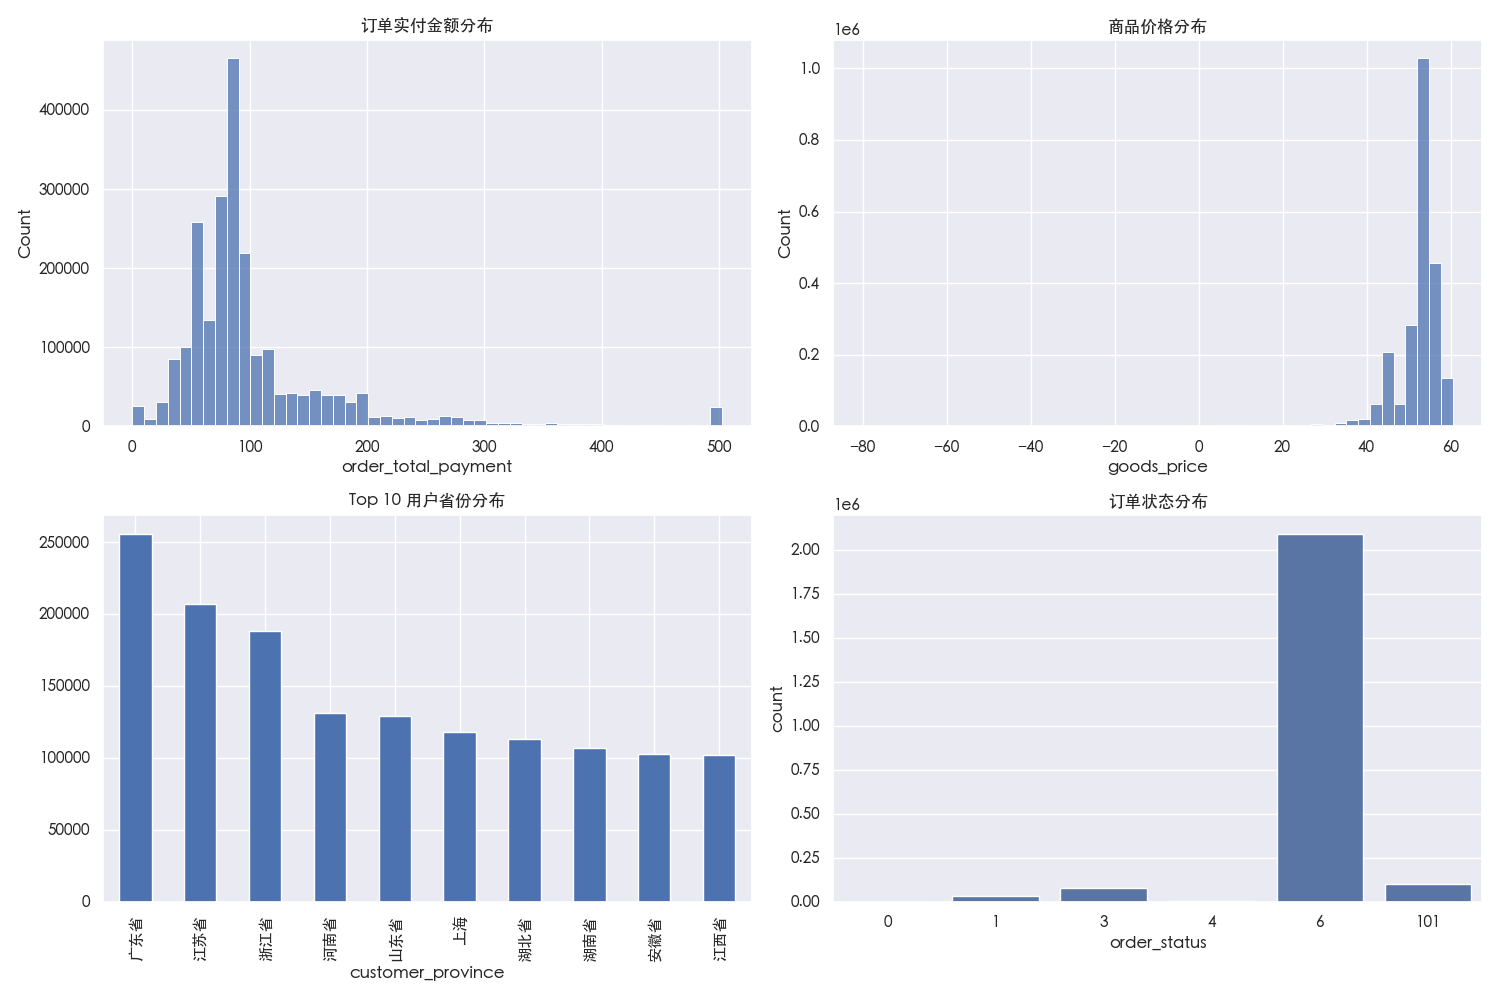
\includegraphics[width=0.9\textwidth]{../analysis/overall_analysis.png}
    \caption{数据集关键特征分布}
    \label{fig:overall_analysis}
    \vspace{1em} % 增加图片和文字之间的间距
    \small
    \textit{注: 图 1 展示了订单金额、商品价格、用户省份和订单状态的分布, 揭示了数据集中用户消费行为集中于低金额订单, 商品价格较为稳定, 地理分布不均, 且交易成功订单占主导.}
\end{figure}

\subsection{不同特征的重要性}

为了评估特征对预测用户未来购买行为的重要性, 我们先基于静态聚合特征构建了用户画像, 并使用LightGBM模型进行简单的训练, 以下是特征重要性分析的结果:

\begin{enumerate}
    \item \textbf{特征工程概述}:
    \begin{itemize}
        \item \textbf{静态聚合特征}: 按 \texttt{customer\_id} 聚合订单和商品相关信息, 包括:
        \begin{itemize}
            \item 订单金额(\texttt{order\_total\_payment}): 均值、总和、最小值、最大值、标准差.
            \item 订单商品数量(\texttt{order\_total\_num}): 均值、总和.
            \item 订单折扣(\texttt{order\_total\_discount}): 均值、总和.
            \item 商品价格(\texttt{goods\_price}): 均值、最小值、最大值、标准差.
            \item 订单总数(\texttt{order\_count}): 总和.
            \item 地理信息(\texttt{customer\_province}, \texttt{customer\_city}): 标签编码.
            \item 时间特征: 最后一次订单距 2013-06-30 的天数(\texttt{days\_since\_last\_order}).
        \end{itemize}
        \item \textbf{标签构建}: 若用户在 2013-07-01 至 2013-07-31 有购买记录, 标签为 1, 否则为 0.
        \item \textbf{数据集划分}: 训练集基于 \texttt{order\_pay\_time <= 2013-06-30}($1,354,575$ 条记录), 验证集基于 \texttt{order\_pay\_time <= 2013-07-31}($1,434,115$ 条记录), 特征缺失值填充为 -999.
    \end{itemize}

    \item \textbf{特征重要性排名} (Top 15, 基于特征分裂增益, 见图 \ref{fig:feature_importance}):
    \begin{itemize}
        \item \texttt{days\_since\_last\_order} (343): 最后一次订单距 2013-06-30 的天数, 排名第一, 表明用户近期活跃度对预测至关重要.
        \item \texttt{customer\_city\_encoded} (267): 城市编码, 地理位置对购买行为有显著影响.
        \item \texttt{goods\_price\_max} (232): 最高商品价格, 反映用户高端消费能力.
        \item \texttt{goods\_price\_min} (199): 最低商品价格, 可能捕捉用户对低价商品的偏好.
        \item \texttt{order\_total\_payment\_min} (180): 最低订单实付金额.
        \item \texttt{customer\_province\_encoded} (179): 省份编码.
        \item \texttt{goods\_price\_mean} (169): 商品平均价格.
        \item \texttt{order\_total\_payment\_sum} (168): 订单实付总金额.
        \item \texttt{order\_total\_payment\_mean} (151): 订单平均实付金额.
        \item \texttt{goods\_price\_std} (150): 商品价格标准差.
        \item \texttt{order\_total\_payment\_std} (145): 订单实付金额标准差.
        \item \texttt{order\_total\_discount\_mean} (132): 平均订单优惠金额.
        \item \texttt{order\_total\_payment\_max} (122): 最高订单实付金额.
        \item \texttt{order\_detail\_goods\_num\_sum} (111): 订单商品总数.
        \item \texttt{customer\_gender\_encoded} (110): 性别编码.
    \end{itemize}

    \begin{figure}[H]
        \centering
        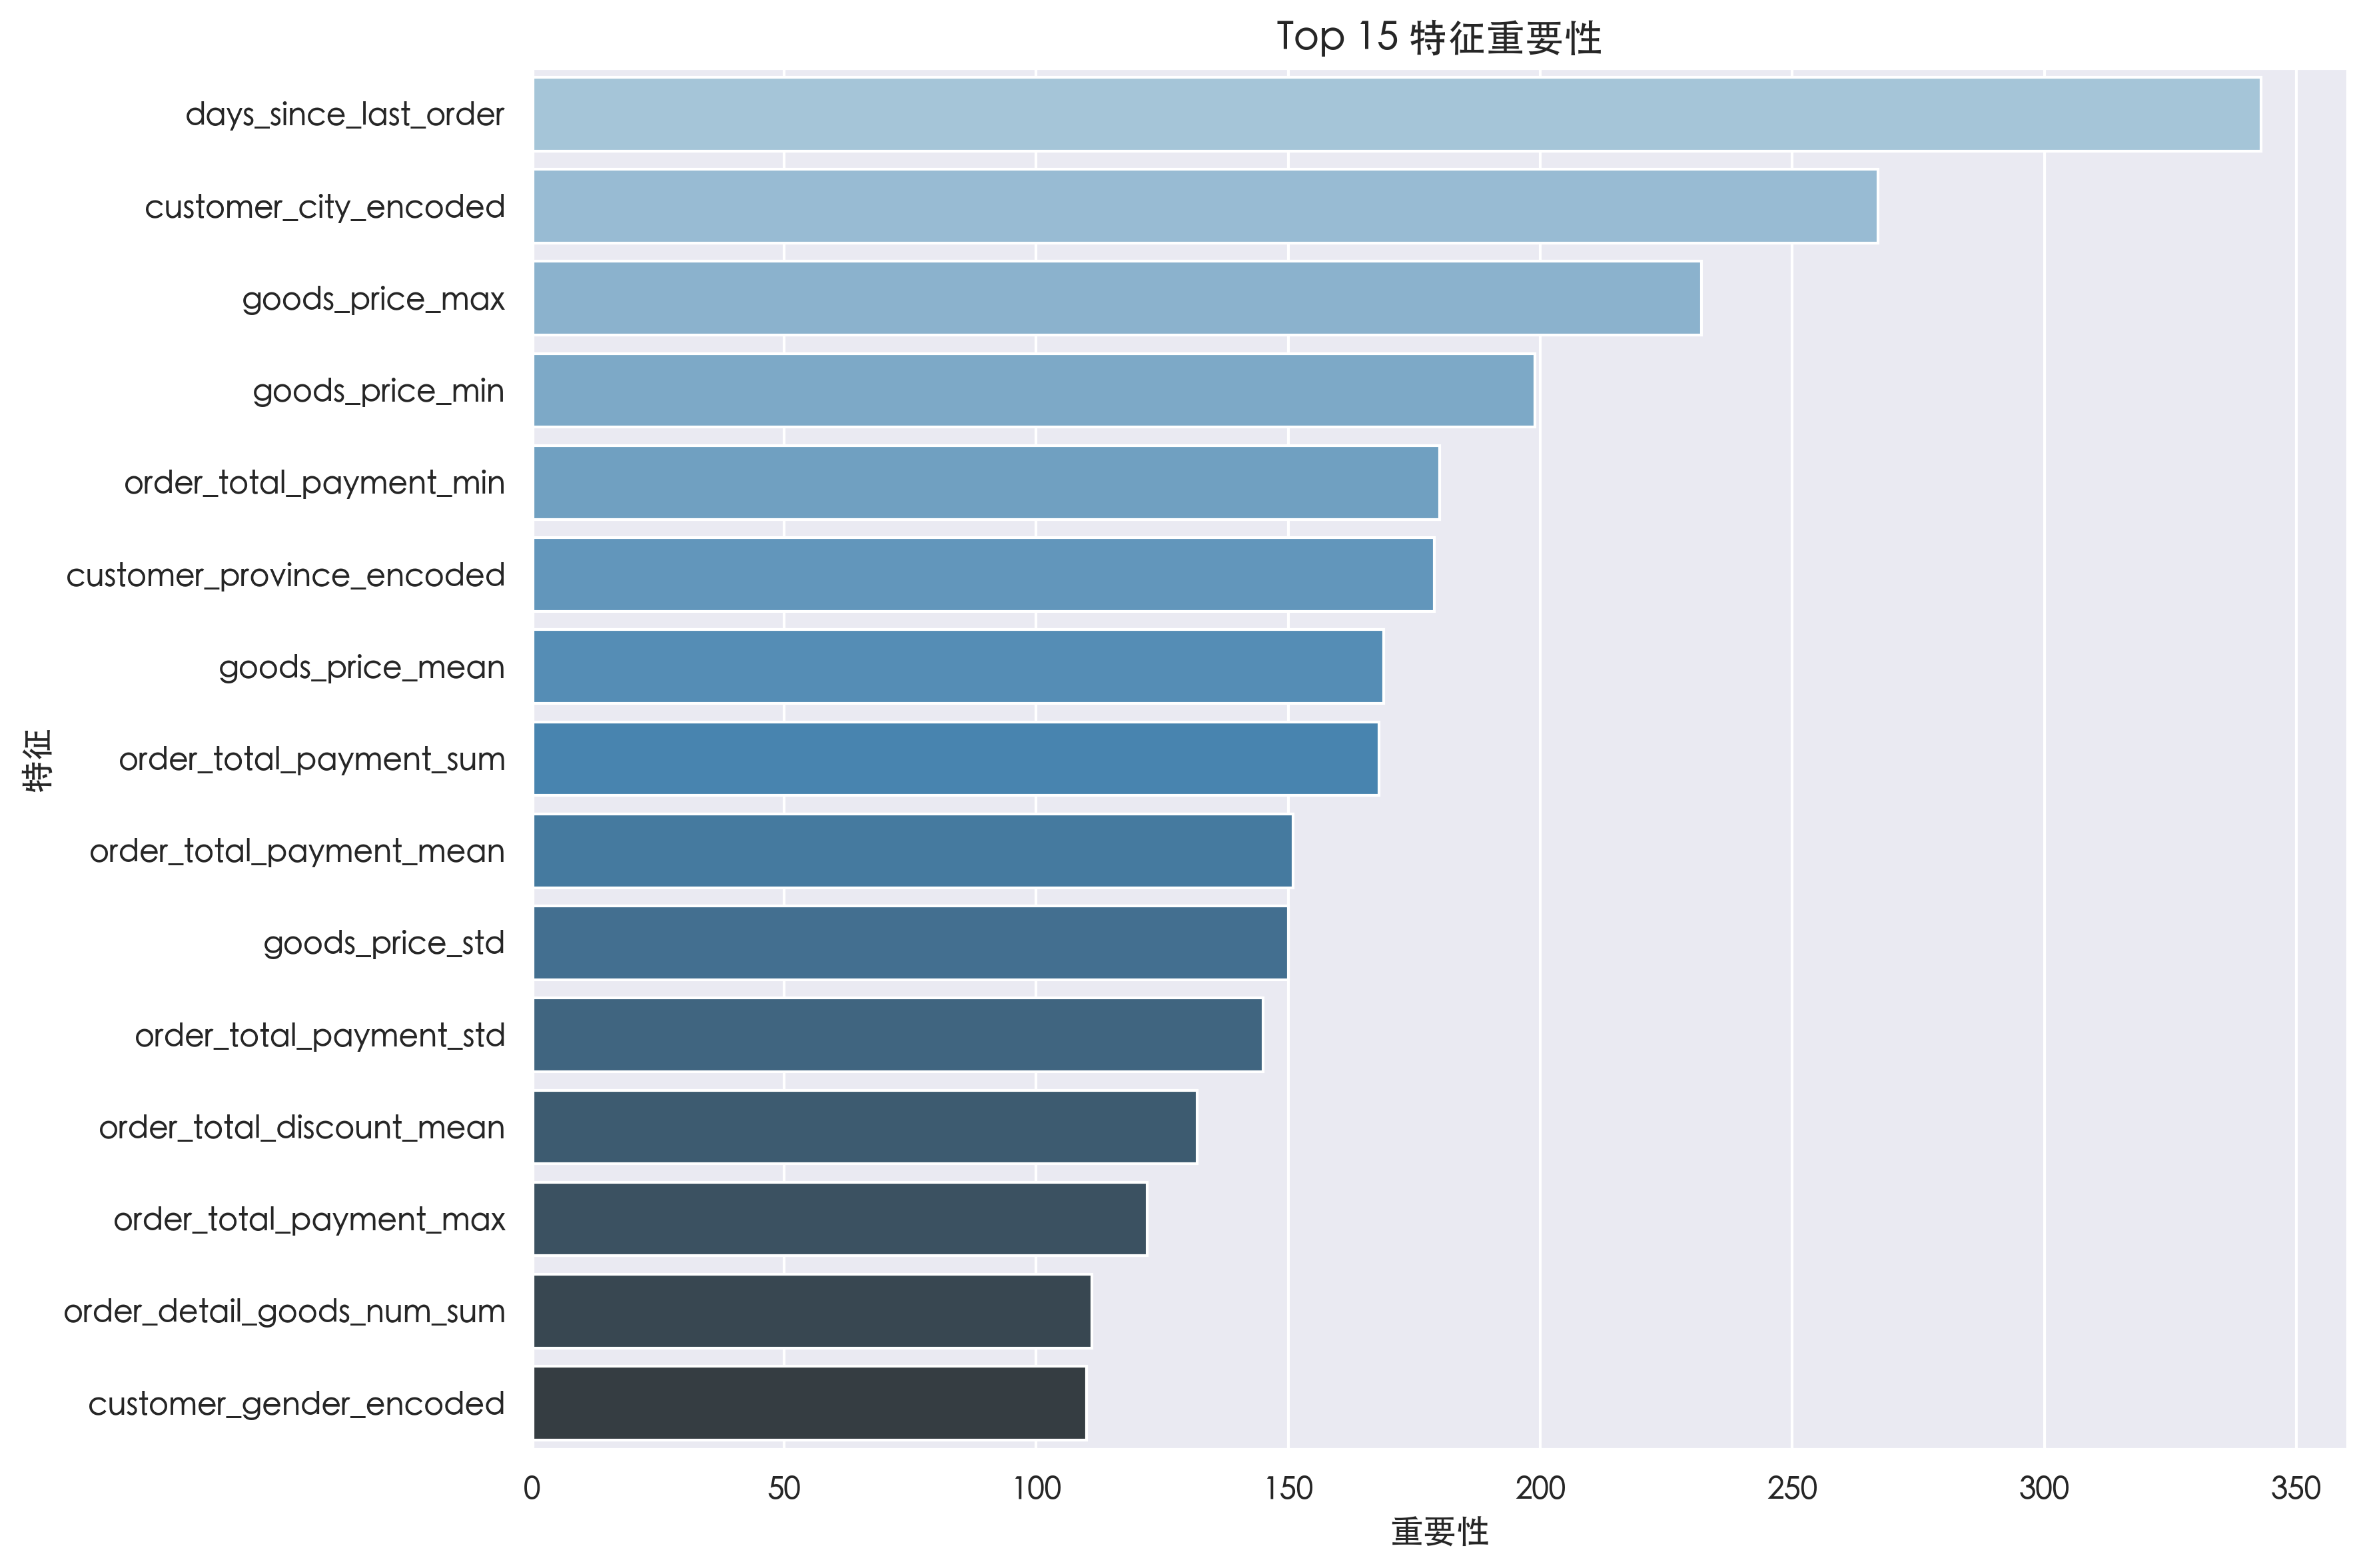
\includegraphics[width=0.8\textwidth]{../analysis/feature_importance.png}
        \caption{特征重要性排名(Top 15)}
        \label{fig:feature_importance}
        \vspace{1em}
        \small
        \textit{注: 图 2 展示了 Top 15 特征的重要性, \texttt{days\_since\_last\_order} 和地理信息占据主导, 消费行为和商品价格相关特征也有显著贡献.}
    \end{figure}

    \item \textbf{分析与洞察}:
    \begin{itemize}
        \item \textbf{时间特征主导}: \texttt{days\_since\_last\_order} 排名第一, 表明用户近期活跃度是预测未来购买的核心指标.
        \item \textbf{地理信息重要}: \texttt{customer\_city\_encoded} 和 \texttt{customer\_province\_encoded} 排名靠前, 表明地理位置对购买行为有显著影响.
        \item \textbf{消费行为特征}: 订单金额和商品价格的相关统计量重要性较高, 反映用户消费能力、购买偏好和价格敏感度是关键预测因子.
        \item \textbf{折扣敏感性}: \texttt{order\_total\_discount\_mean} 排名靠前, 表明优惠对部分用户的购买决策有影响.
        \item \textbf{性别特征潜力}: \texttt{customer\_gender\_encoded} 尽管数据缺失严重, 仍显示一定重要性.
    \end{itemize}
\end{enumerate}


\section{特征工程与训练集验证集划分}
项目的核心任务是预测 \texttt{customer\_id} 在未来是否会产生购买行为. 我们的特征工程将围绕 \texttt{customer\_id} 进行, 聚合每个用户的历史行为信息.

我们采用了两种互补的特征工程方法, 由 \texttt{config.data.feature\_method} 参数控制:
\begin{enumerate}
    \item \textbf{静态聚合特征 (\texttt{agg})}: 该方法将每个用户在特定时间点之前的所有历史行为数据进行聚合, 生成一组描述用户整体画像的统计特征.
    \item \textbf{动态时序特征 (\texttt{time})}: 该方法将用户的购买和支付行为看作时间序列, 通过在不同长度的时间窗口上进行滑窗统计, 捕捉用户近期行为的动态变化趋势.
\end{enumerate}

\subsection{静态聚合特征}
静态特征主要由 \texttt{preprocess\_agg} 函数实现, 为每个 \texttt{customer\_id} 生成一个截至某个时间点的全局行为表征. 具体构建的特征如下:
\begin{enumerate}
    \item \textbf{最后一次行为特征}: 提取用户最后一次交互的各类信息, 如 \texttt{goods\_id\_last}, \texttt{order\_amount\_last} 等.
    \item \textbf{聚合特征}: 对数值型特征计算统计量.
    \begin{itemize}
        \item 对商品价格 (\texttt{goods\_price}) 计算其最小值, 最大值, 均值和标准差.
        \item 对订单支付金额 (\texttt{order\_total\_payment}) 计算其最小值、最大值、均值和标准差.
        \item 对订单商品总数 (\texttt{order\_total\_num})、订单折扣 (\texttt{order\_detail\_discount}) 等计算均值和总和.
    \end{itemize}
    \item \textbf{计数类特征}: 如 \texttt{order\_count}, \texttt{goods\_count}.
    \item \textbf{其他聚合特征}:
    \begin{itemize}
        \item \texttt{discount}: 通过 \texttt{order\_detail\_amount\_last / order\_detail\_payment\_last} 计算用户最近一次购买的折扣力度.
        \item \textbf{时间处理}:
        \begin{itemize}
            \item 将最后支付时间分解为月、日、星期几等多个维度.
            \item 计算时间差, 将绝对时间转化为相对时间间隔.
            \item 计算商品从上架到下架的持续时间 \texttt{goods\_time\_diff}.
        \end{itemize}
    \end{itemize}
    \item \textbf{空值与无穷值处理}: 统一使用 $-999$ 填充所有 \texttt{NaN} 值.
\end{enumerate}

\subsection{动态时序特征}
为了更精细地捕捉用户行为的时序动态性, 我们设计了 \texttt{generate\_timeseries\_features} 函数, 通过\textbf{滑动窗口法}构建了一系列时序特征.
\begin{enumerate}
    \item \textbf{支付行为时间序列特征}:
    \begin{itemize}
        \item \textbf{时间窗口}: 选取了14天、30天、60天、91天作为滑窗长度.
        \item \textbf{衰减加权统计}: 计算了窗口内每日支付额的\textbf{衰减加权均值}(\texttt{payment\_mean\_\{T\}d\_decay}), 衰减系数为0.9.
        \item \textbf{常规统计}: 计算了窗口内的支付总额 (\texttt{\_sum}) 和最大单日支付 (\texttt{\_max}).
        \item \textbf{行为频率特征}: 窗口内消费天数、最近/首次消费距今时间.
        \item \textbf{跨周期比较}: 计算了当前窗口与上一周同一窗口的统计量.
        \item \textbf{月度聚合}: 聚合了过去3个月的消费总额.
    \end{itemize}
    \item \textbf{购买商品数量时间序列特征}:
    \begin{itemize}
        \item \textbf{时间窗口}: 选取了21天、49天、84天作为滑窗长度.
        \item \textbf{特征类别}: 与支付行为特征类似, 计算了购买商品总数、均值、最大值, 购买天数, 以及最近/最远购买日期间隔等.
        \item \textbf{近似月度聚合}: 聚合了过去3个周期(每28天为一个周期)的购买商品总数.
    \end{itemize}
\end{enumerate}

\subsection{Label构建}
预测任务是判断用户在未来一个月内是否会购买. 目标变量 \texttt{label} 的构建逻辑如下:
$$
\text{label}_i = 
\begin{cases} 
    1, & \text{if customer } i \text{ made a purchase in } (T, T + 1\text{ month}] \\
    0, & \text{otherwise} 
\end{cases}
$$
其中 $T$ 是特征提取的时间截止点.

\subsection{数据集划分与最终处理}
我们采用了基于时间的滚动窗口来切分数据集.
\begin{enumerate}
    \item \textbf{训练集}:
    \begin{itemize}
        \item \textbf{特征区间}: \texttt{order\_pay\_time} $\le$ \texttt{2013-06-30}
        \item \textbf{标签区间}: \texttt{2013-07-01} 至 \texttt{2013-07-31}
    \end{itemize}
    \item \textbf{验证集}:
    \begin{itemize}
        \item \textbf{特征区间}: \texttt{order\_pay\_time} $\le$ \texttt{2013-07-31}
        \item \textbf{标签区间}: \texttt{2013-08-01} 至 \texttt{2013-08-31}
    \end{itemize}
    \item \textbf{测试集}:
    \begin{itemize}
        \item \textbf{特征区间}: \texttt{order\_pay\_time} $\le$ \texttt{2013-08-31}
        \item \textbf{标签区间}: 无 (用于线上预测)
    \end{itemize}
\end{enumerate}
最后, 对类别特征使用 \texttt{sklearn.preprocessing.LabelEncoder} 进行标签编码, 保证训练集、验证集和测试集编码的一致性.

\section{算法实现}
\subsection{总体框架}
我们设计了一套统一的、可扩展的算法框架.
\begin{enumerate}
    \item \textbf{模型基类 (\texttt{model.py})}: 定义了基类 \texttt{BaseModel}, 规范了所有模型类必须的 \texttt{train} 和 \texttt{predict} 两个接口.
    \item \textbf{训练与预测脚本 (\texttt{train.py})}: 项目的总控制脚本.
    \begin{itemize}
        \item \textbf{配置管理}: 使用 \texttt{Hydra} 库来管理所有配置.
        \item \textbf{模型工厂}: \texttt{get\_model} 函数根据配置实例化对应的模型对象.
        \item \textbf{训练流程}: \texttt{train} 函数负责加载数据、调用模型训练方法.
        \item \textbf{预测流程}: \texttt{predict} 函数负责加载模型、生成预测结果.
    \end{itemize}
\end{enumerate}

\subsection{模型实现详情}
我们共实现了四种不同的模型.
\begin{enumerate}
    \item \textbf{回归模型 (手动实现)}: 使用 \texttt{Numpy} 从零开始实现逻辑回归.
    \begin{itemize}
        \item \textbf{网络结构}: 采用梯度下降算法优化权重. 权重更新公式为:
        $$ W_{new} = W_{old} - \alpha \frac{1}{m} X^T(\sigma(XW) - y) $$
        其中 $\sigma$ 是 Sigmoid 函数.
        \item \textbf{模型封装 (\texttt{RegModel})}: 在训练前对特征进行标准化处理.
    \end{itemize}
    
    \item \textbf{XGBoost}: 封装 \texttt{xgboost} 库中的 \texttt{XGBClassifier}.
    \begin{itemize}
        \item \textbf{超参数配置}: 通过 \texttt{Hydra} 配置文件传入.
        \item \textbf{训练与评估}: 调用 \texttt{.fit()} 方法, 传入验证集进行监控和早停.
        \item \textbf{模型保存}: 保存为 \texttt{.json} 文件.
    \end{itemize}
    
    \item \textbf{LightGBM}: 封装 \texttt{lightgbm} 库中的 \texttt{LGBMClassifier}.
    \begin{itemize}
        \item \textbf{超参数配置}: 同样由外部配置传入.
        \item \textbf{训练与评估}: 流程与 XGBoost 类似.
        \item \textbf{模型保存}: 通过 \texttt{joblib} 库序列化为 \texttt{.joblib} 文件.
    \end{itemize}

    \item \textbf{多层感知机 (Multi-Layer Perceptron)}: 使用 \texttt{PyTorch} 构建.
    \begin{itemize}
        \item \textbf{网络结构}: 多个可配置的隐藏层组成, 每个隐藏层是 "Linear + BN + ReLU + Dropout" 的模块, 采用 Kaiming 初始化.
        \item \textbf{模型封装 (\texttt{MLPModel})}: 使用 \texttt{Adam} 优化器和 \texttt{BCEWithLogitsLoss} 损失函数. 训练循环中包含验证评估和模型保存逻辑.
    \end{itemize}
\end{enumerate}

\section{结果分析}
我们以 \textbf{AUC} 作为核心评估指标, 从特征工程和算法模型两个角度展开讨论. 我们设计了三套特征工程方案: \textbf{\texttt{agg}}(静态聚合特征)、\textbf{\texttt{time}} (动态时序特征) 和 \textbf{\texttt{both}} (两者结合).

\subsection{结果}

\begin{figure}[H]
    \centering
    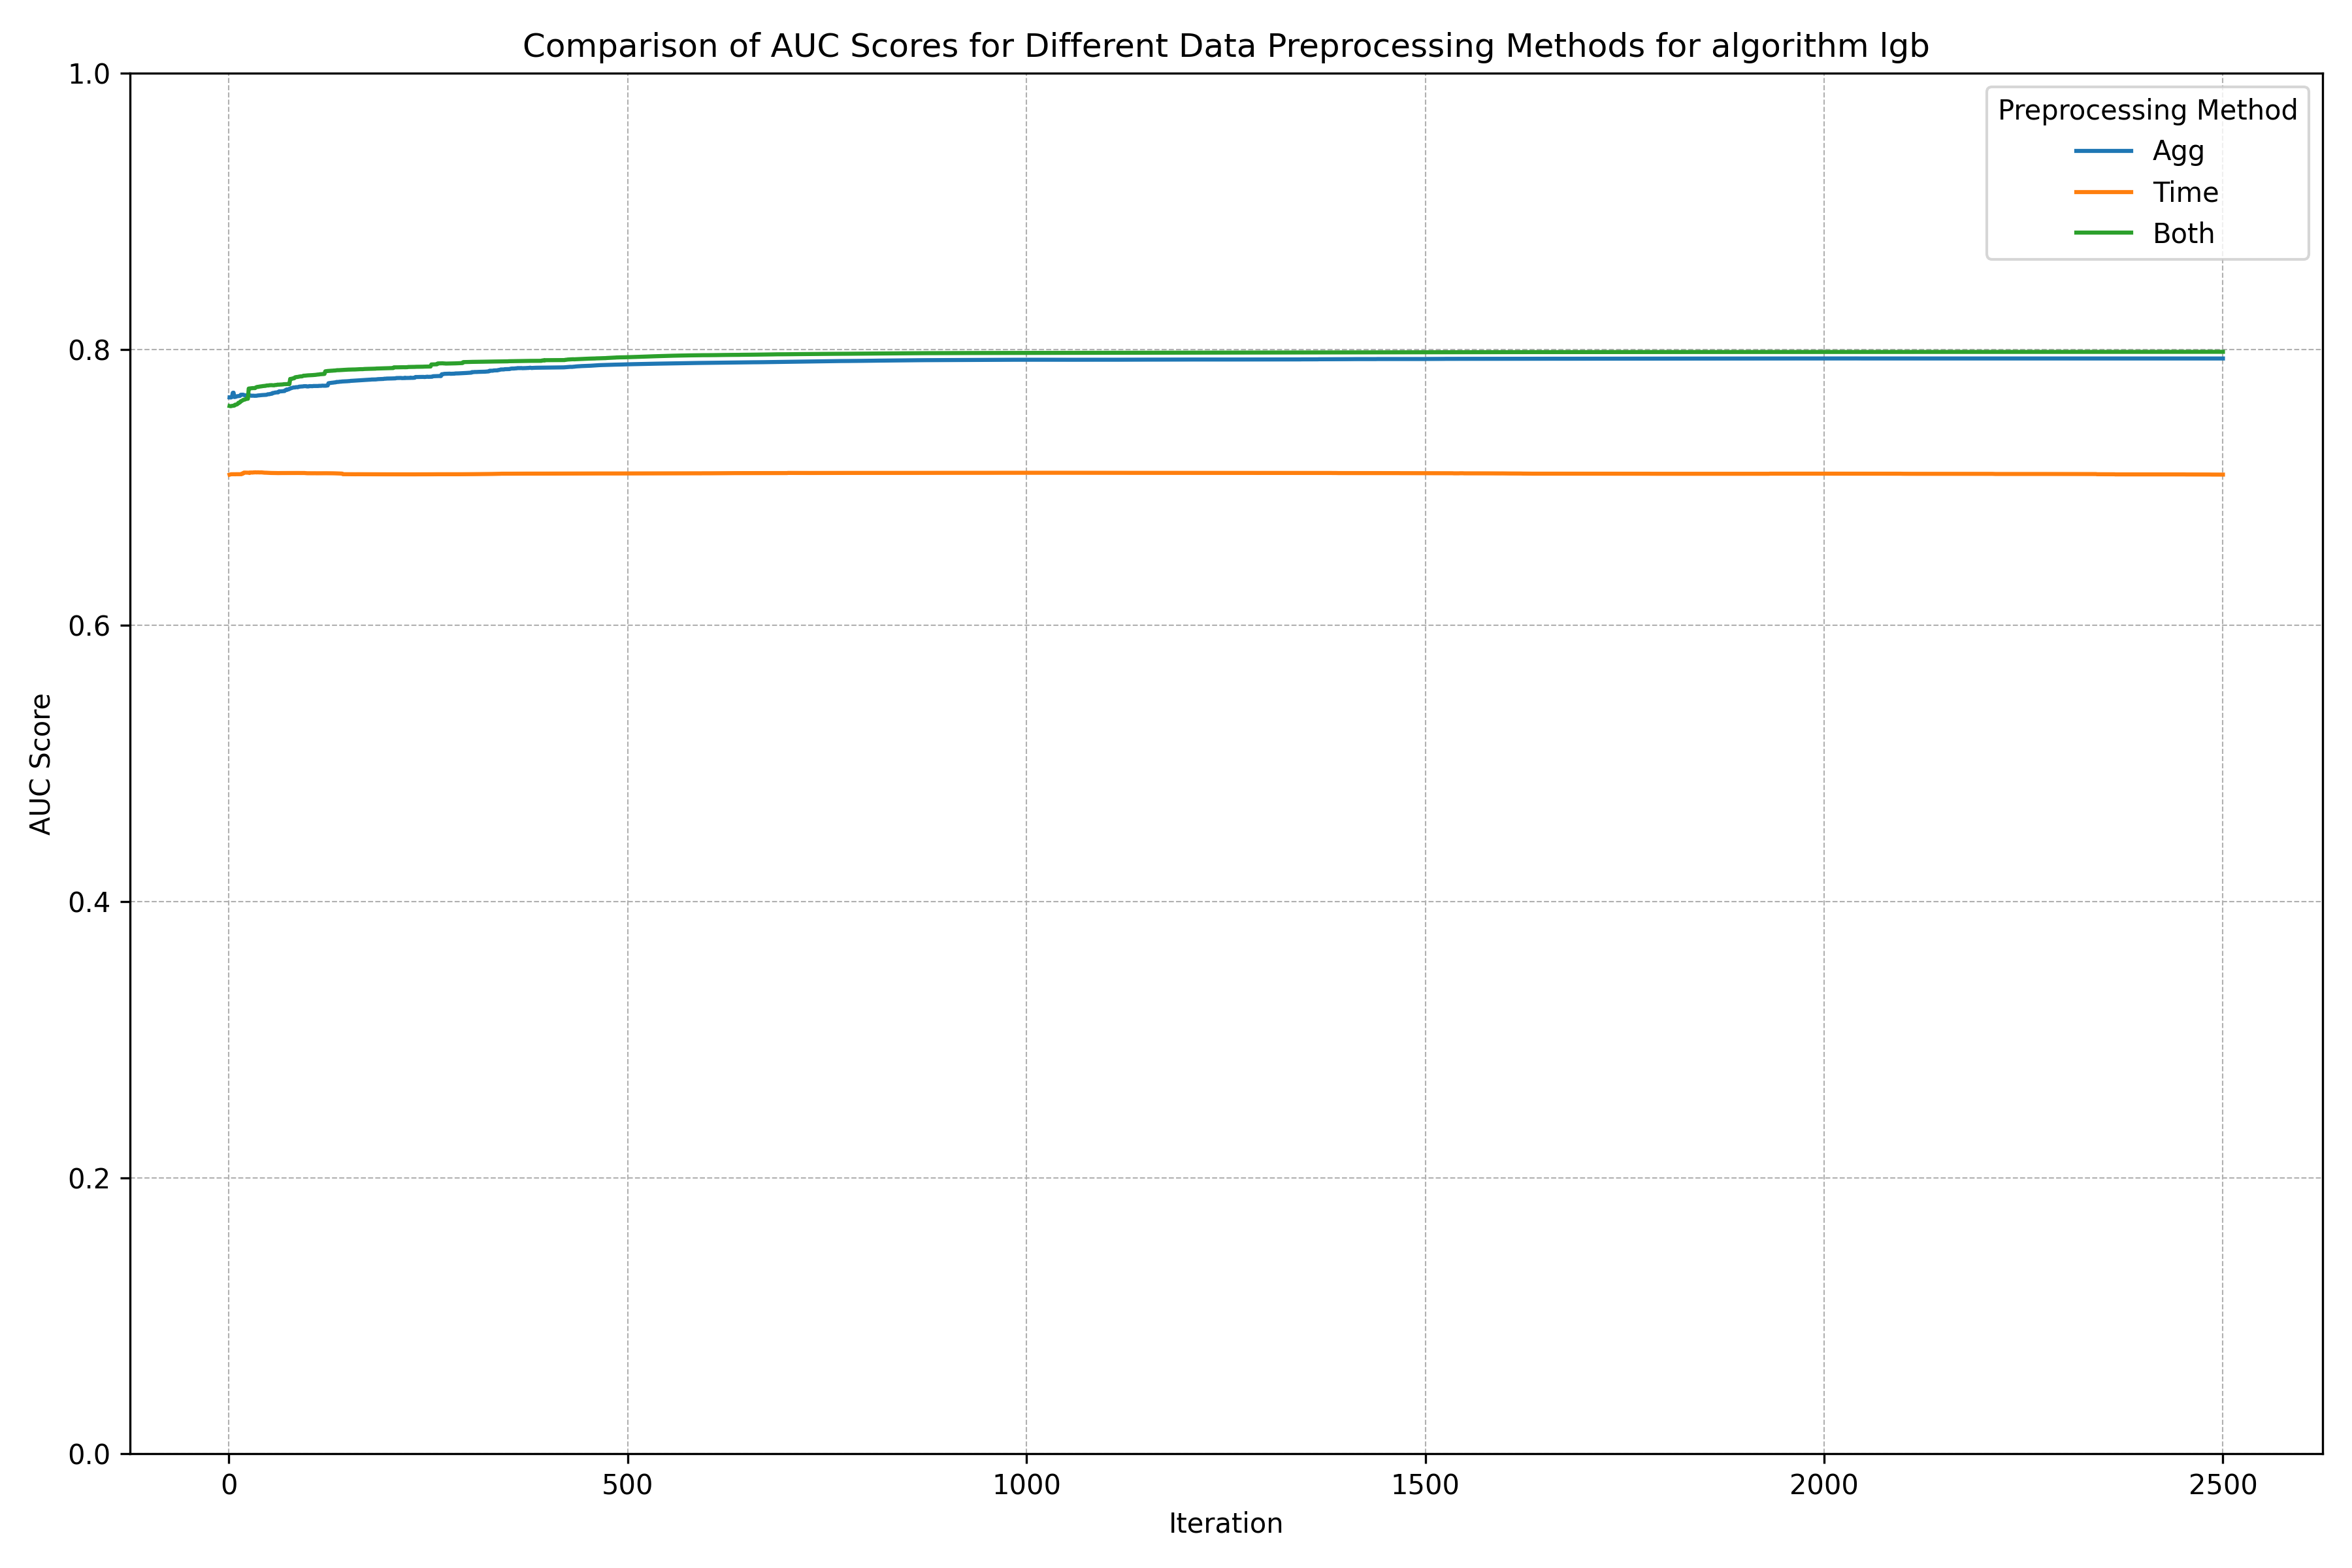
\includegraphics[width=0.7\textwidth]{../figs/lgbauc.png}
    \caption{LGBM 模型在不同特征集上的AUC表现}
    \label{fig:lgbauc}
\end{figure}

\begin{figure}[H]
    \centering
    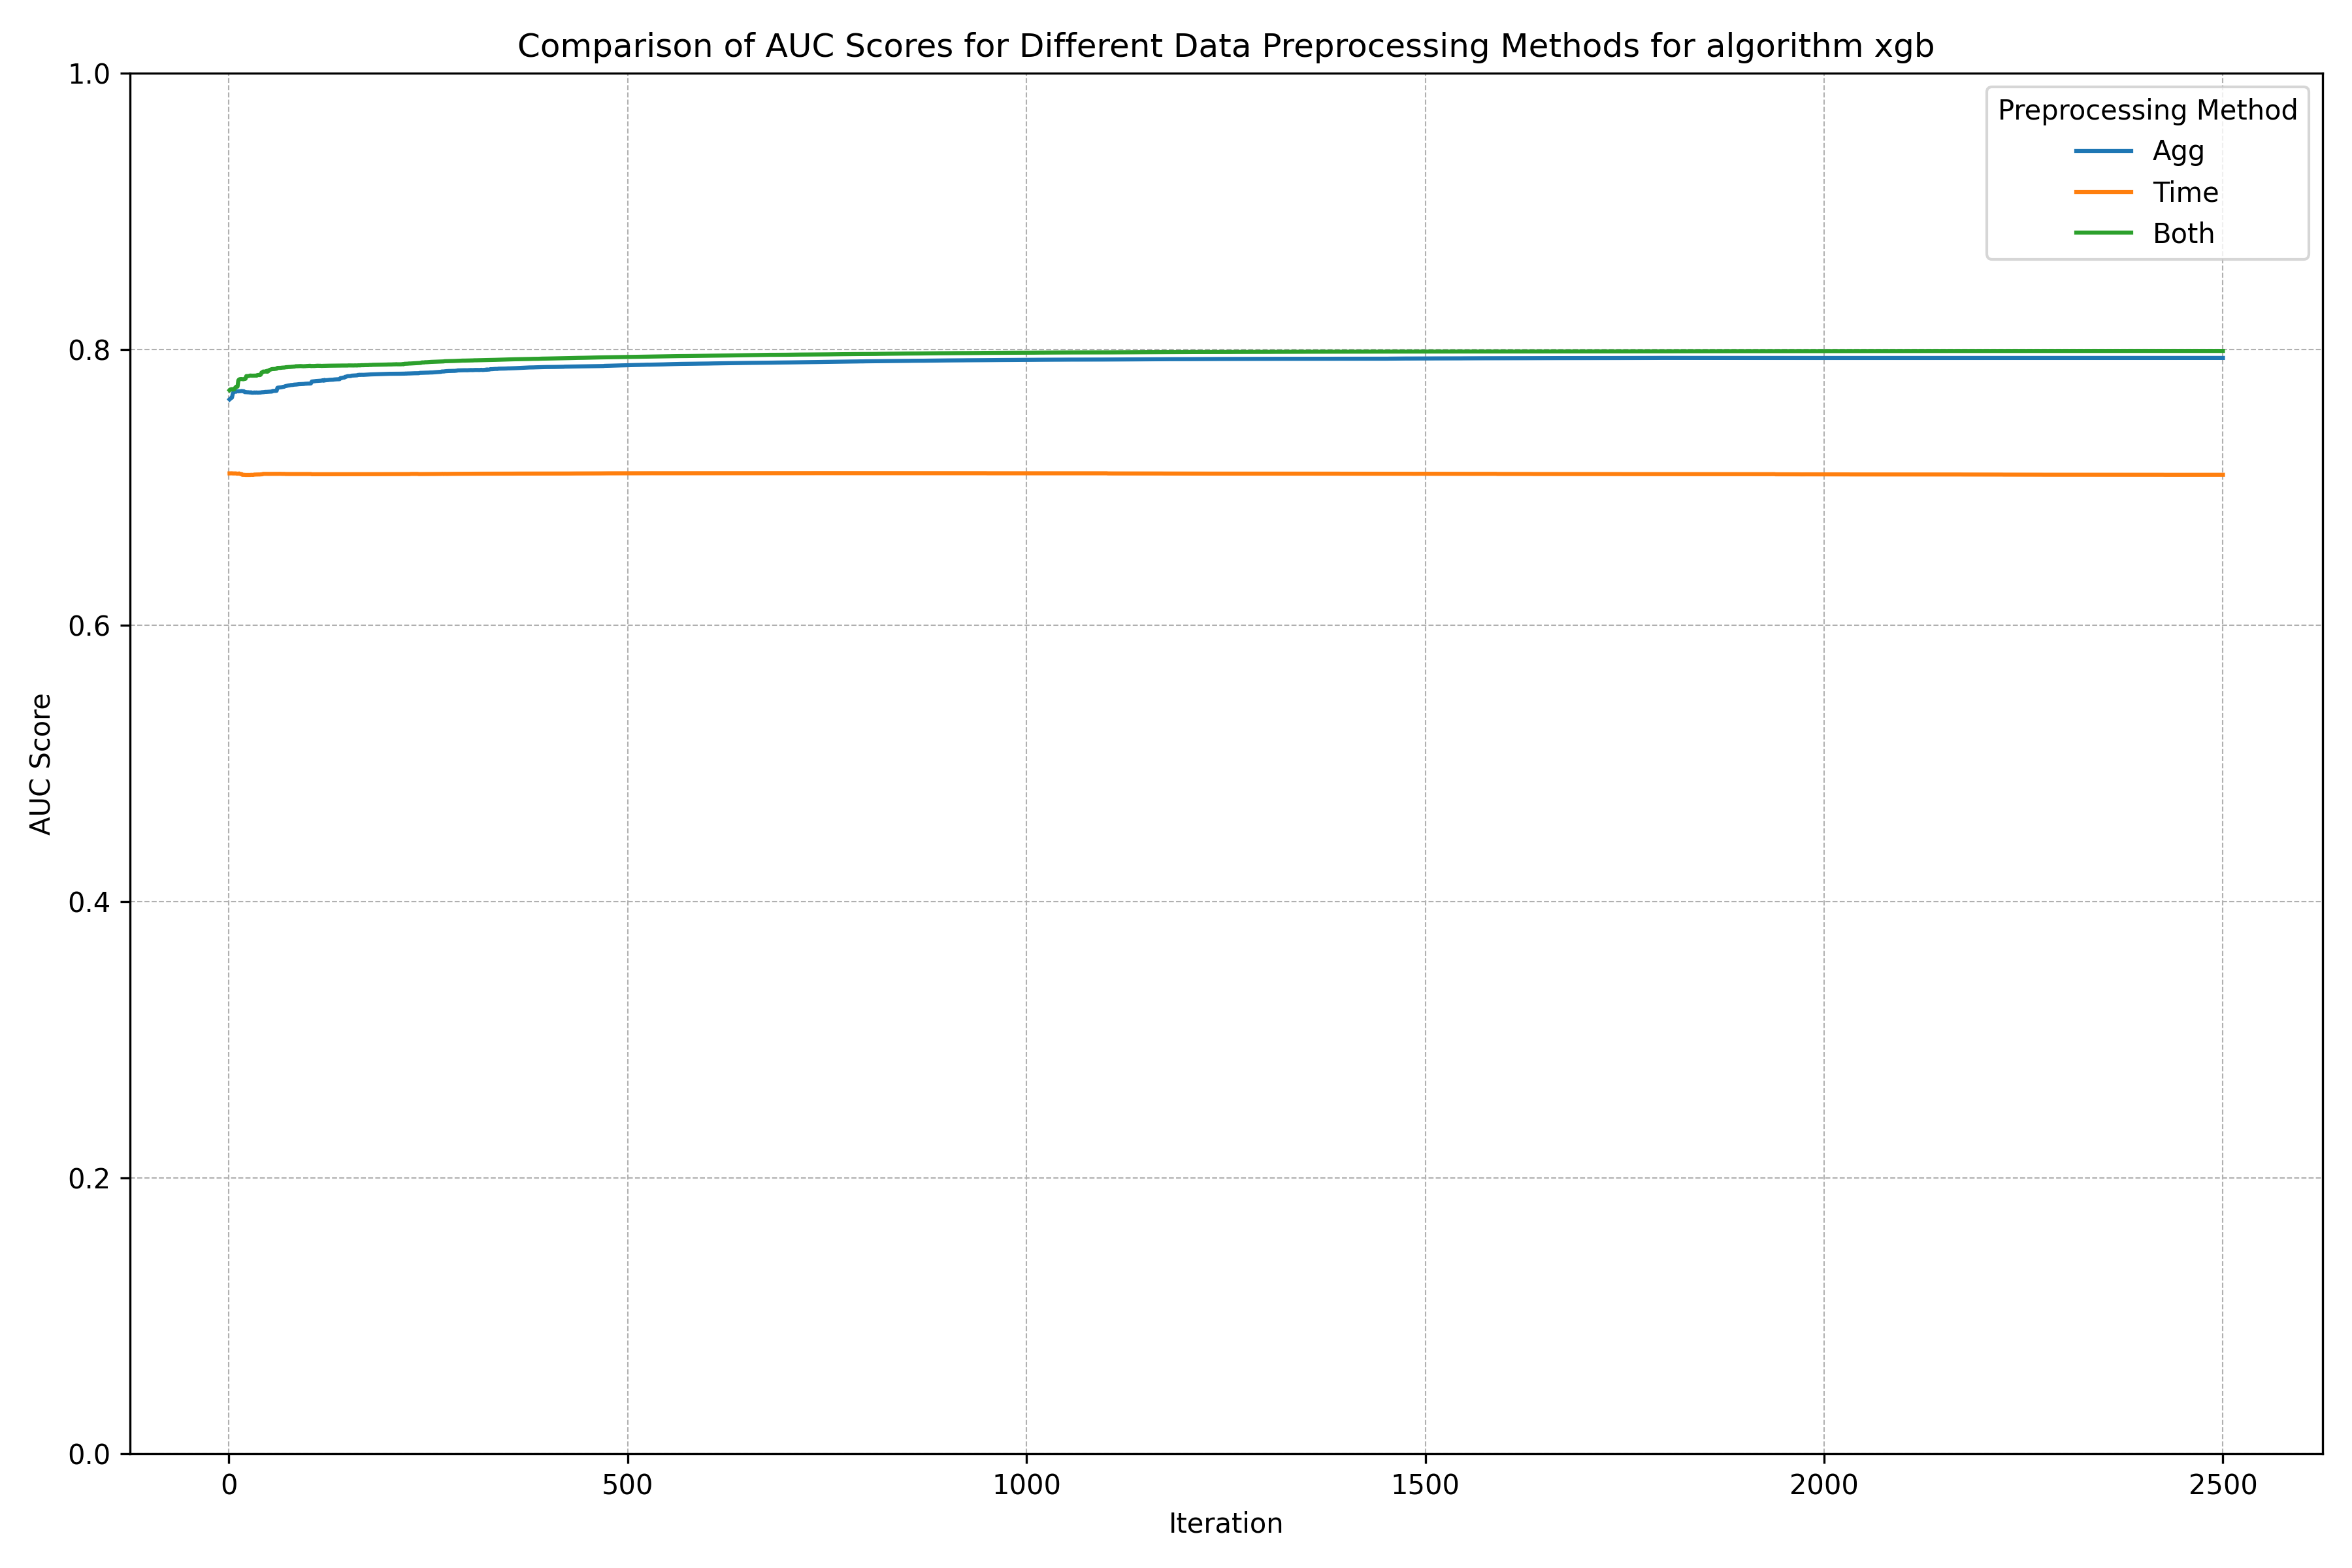
\includegraphics[width=0.7\textwidth]{../figs/xgbauc.png}
    \caption{XGBoost 模型在不同特征集上的AUC表现}
    \label{fig:xgbauc}
\end{figure}

\begin{figure}[H]
    \centering
    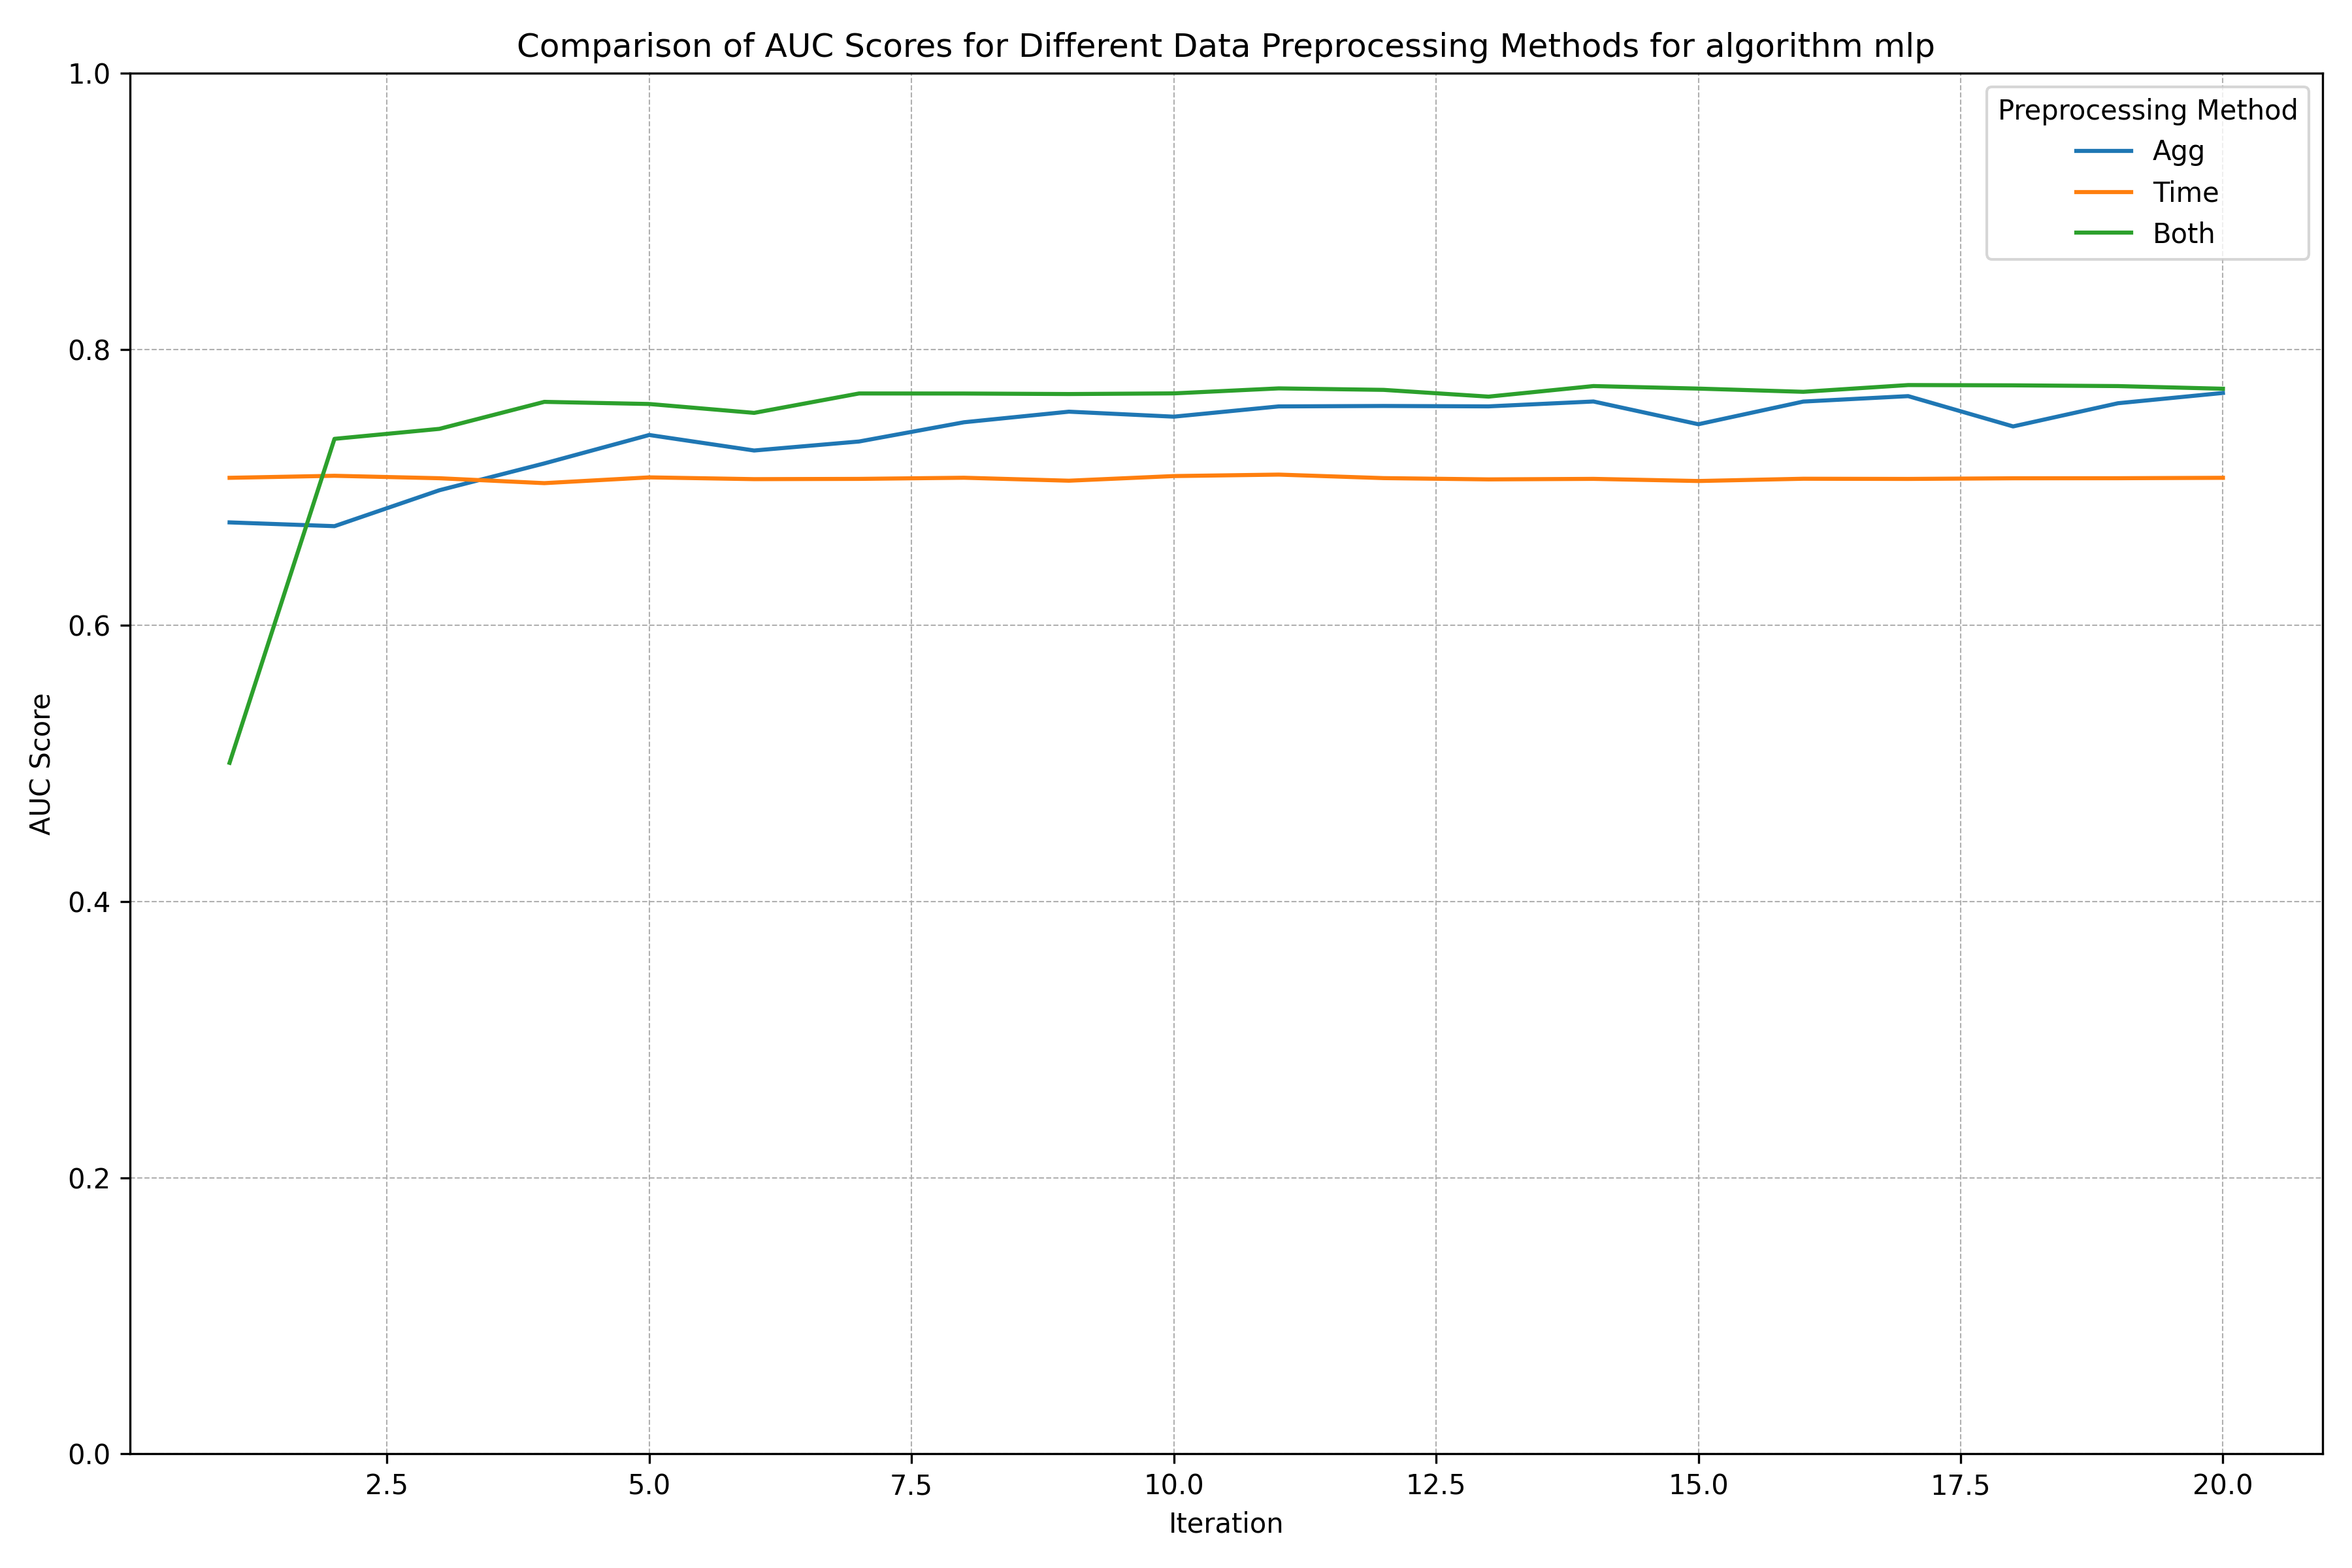
\includegraphics[width=0.7\textwidth]{../figs/mlpauc.png}
    \caption{MLP 模型在不同特征集上的AUC表现}
    \label{fig:mlpauc}
\end{figure}

\begin{figure}[H]
    \centering
    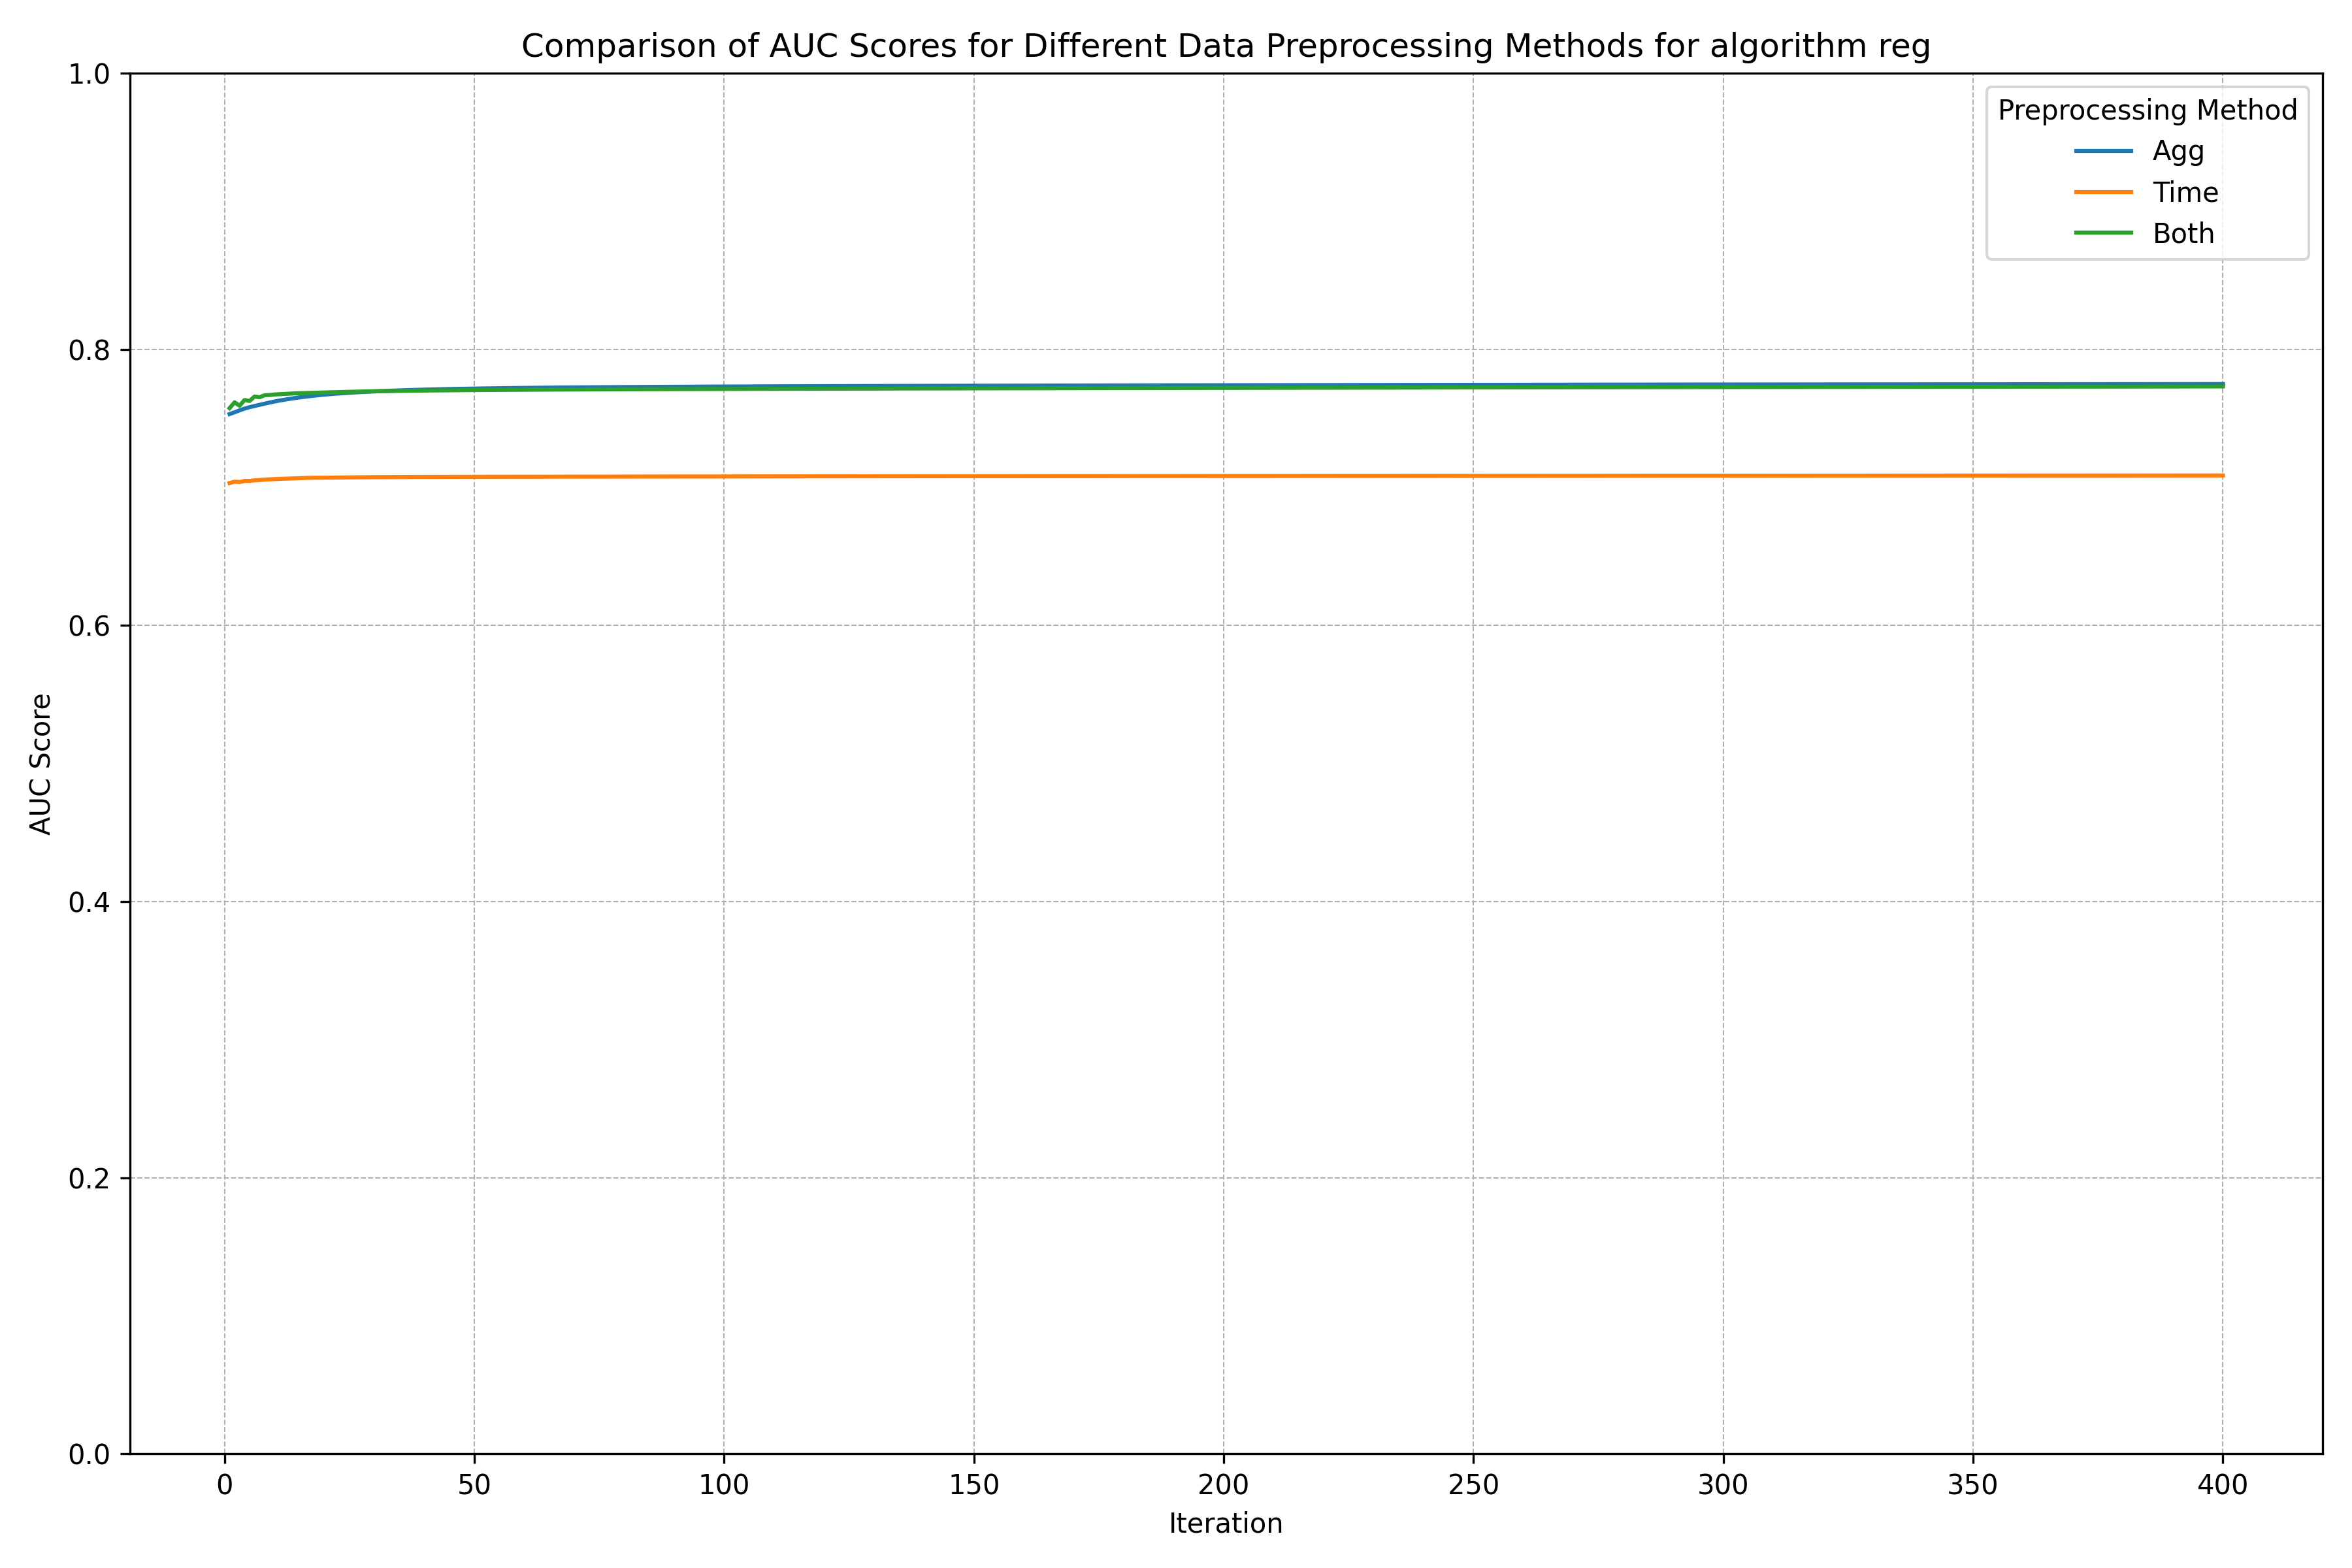
\includegraphics[width=0.7\textwidth]{../figs/regauc.png}
    \caption{逻辑回归模型在不同特征集上的AUC表现}
    \label{fig:regauc}
\end{figure}

\subsection{特征工程影响}
综合四张图表, 我们可以观察到高度一致且清晰的规律:
\begin{enumerate}
    \item \textbf{性能}: 在XGB, LGB, MLP模型上, 特征集的表现排序均为: \textbf{\texttt{both} > \texttt{agg} >> \texttt{time}}. 在Reg模型上, 后期表现 \textbf{\texttt{agg} > \texttt{both}}.
    \item \textbf{收敛}: 使用 \texttt{time} 特征集时, 所有模型的学习曲线都表现为一条近乎水平的直线. 使用 \texttt{agg} 和 \texttt{both} 特征集时, 模型表现出健康的学习趋势.
\end{enumerate}

\textbf{影响分析}:
\begin{itemize}
    \item \textbf{为什么 \texttt{time} 特征效果不佳?} \texttt{time} 主要刻画了用户行为的时序特征, 缺乏行为的主体信息. 模型仅凭这些信息, 难以了解用户固有属性, 导致预测能力非常有限. 同时时序特征非常\textbf{稀疏}, \textbf{噪音}极大.
    \item \textbf{为什么 \texttt{agg} 特征有稳健表现?} \texttt{agg} 构建的是一个用户的\textbf{长期、稳定的画像}, 不容易被短期的异常行为所干扰.
    \item \textbf{为什么 \texttt{both} 特征能取得最佳效果?} \texttt{both} 特征集融合了长期静态画像(\texttt{agg})和近期行为动态趋势(\texttt{time}), 使得模型既能把握用户的本质, 又能捕捉其状态的边际变化.
    \item \textbf{为什么对\texttt{reg}模型, \texttt{agg}比\texttt{both}表现更好?} 很可能是由于\textbf{噪声}特征的引入所导致的. 线性模型必须为每一个输入特征分配权重, 新增的含噪时序特征损害了从 \texttt{agg} 特征中学到的、更强大的模式, 造成了轻微的\textbf{过拟合}.
\end{itemize}

\subsection{算法影响}
四种算法的性能形成了两个明显的梯队:
\begin{itemize}
    \item \textbf{树模型}: XGBoost 和 LightGBM表现非常接近, AUC值均在 $0.798$ 左右.
    \item \textbf{MLP和Reg}: 逻辑回归和 MLP表现也较为接近, AUC值在 $0.77$ 左右.
\end{itemize}

\textbf{影响分析}:
\begin{itemize}
    \item \textbf{为什么梯度提升树(XGB/LGB)表现最佳?} GBDT算法在处理表格类数据时具有天然优势, 包括高效的非线性关系捕获、对特征缩放不敏感和强鲁棒性.
    \item \textbf{为什么 MLP 和 Reg 表现稍逊?} \textbf{Reg}作为一个\textbf{线性模型}, 难以捕捉非线性关系. \textbf{MLP}虽然理论上可以逼近任意复杂函数, 但在有限的表格数据上, 其优化和调参难度较大, 且特征交互的捕捉不如树模型直接有效. 在本实验中, MLP甚至微弱地输给了逻辑回归, 可能表明对于当前特征集, 复杂的非线性组合并未带来超额收益.
\end{itemize}

\subsection{不同特征的影响}
我们将不同特征的权重可视化之后得到后面的图(图 \ref{fig:xgb_both} 至 \ref{fig:xgb_time}). 从中我们可以看出:
\begin{enumerate}
    \item \textbf{近期消费行为是最强的信号}: 用户近期支付行为相关的特征, 尤其是带时间衰减的加权平均值(\texttt{payment\_mean\_91d\_decay}), 占据了极高的重要性.
    \item \textbf{用户身份与状态占据稳固而可靠的地位}: 用户的静态、长期属性, 特别是会员状态(\texttt{member\_status\_last})和历史购买总数(\texttt{order\_count}), 是模型做出稳健判断的基石.
    \item \textbf{现象解析}: 虽然\texttt{agg}和\texttt{both}性能接近, 但是\texttt{both}中重要性高的指标却是\texttt{time}中的. 这是因为 \texttt{agg} 已经完成了绝大部分预测任务, \texttt{time} 特征只是在 \texttt{agg} 的基础上进行“精修”和“纠错”. 当两个用户的\texttt{agg}特征几乎一样时, \texttt{time} 特征提供了决定性的证据来区分他们, 因此模型给予了它极高的权重, 但它只在这些疑难案例上起作用, 故对总AUC的提升不大.
\end{enumerate}

\begin{figure}[H]
    \centering
    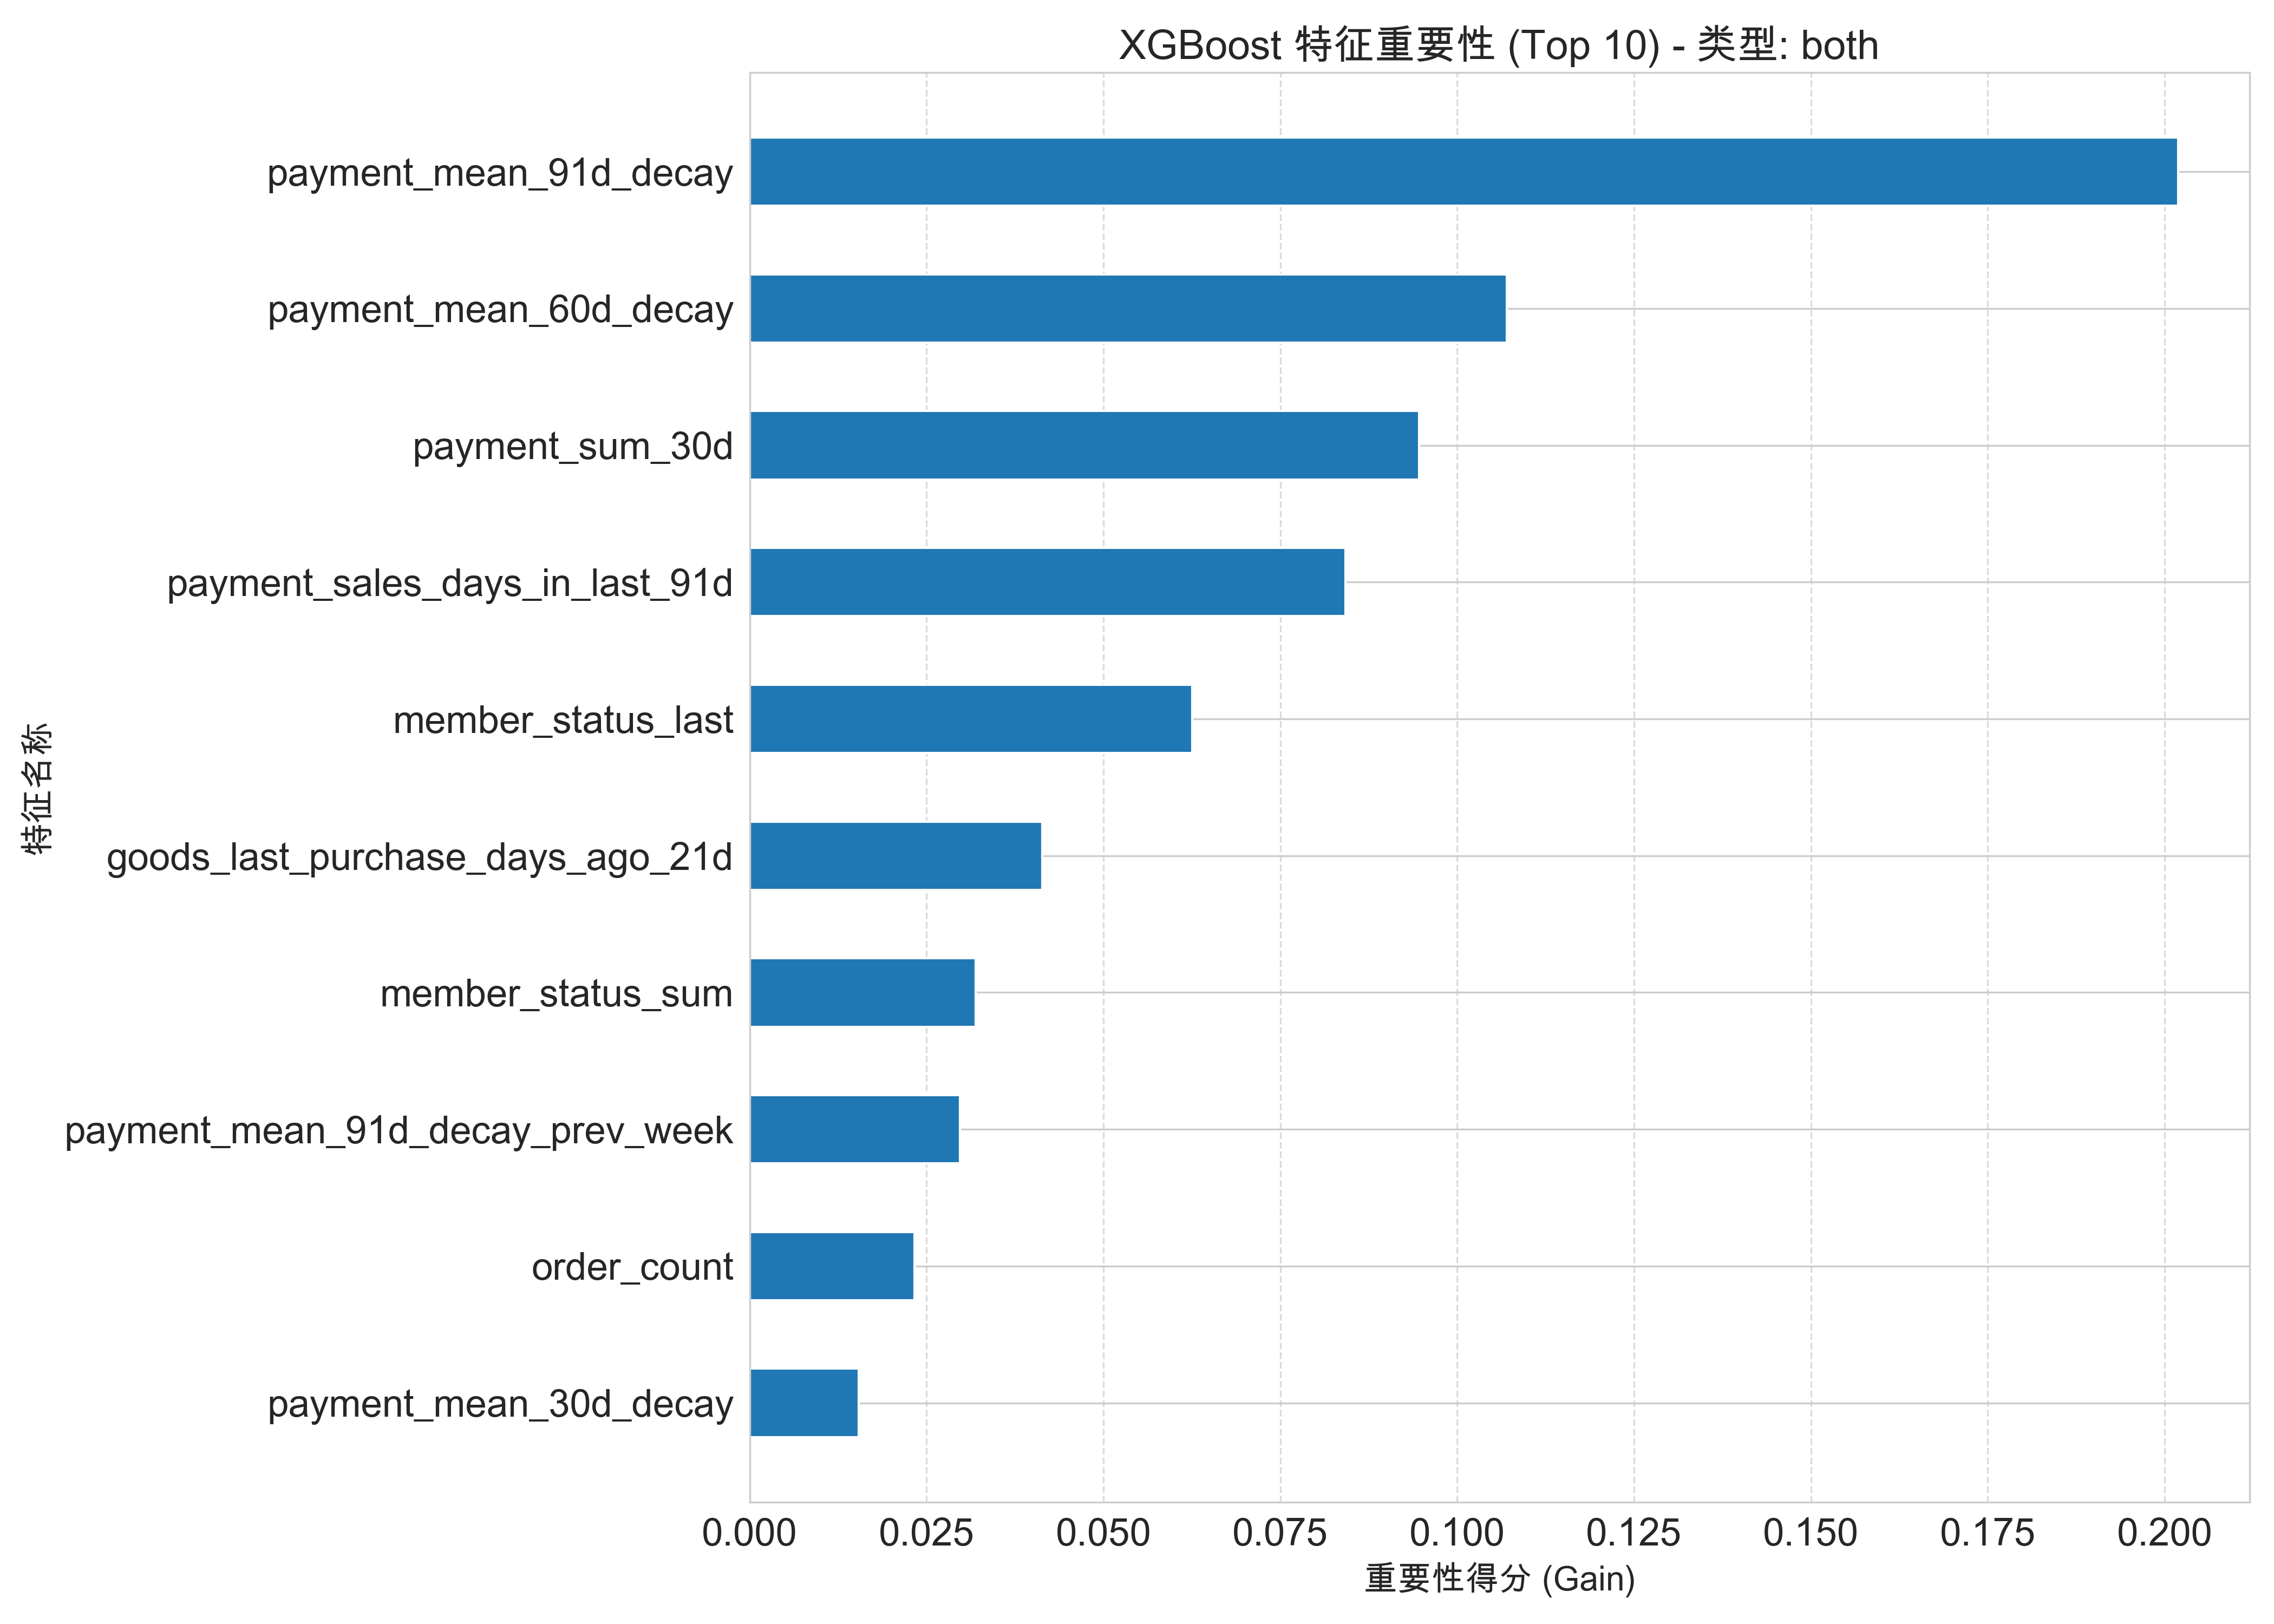
\includegraphics[width=\textwidth]{../analysis/xgb_both_feature_importance.png}
    \caption{XGBoost模型在\texttt{both}特征集上的特征重要性}
    \label{fig:xgb_both}
\end{figure}

\begin{figure}[H]
    \centering
    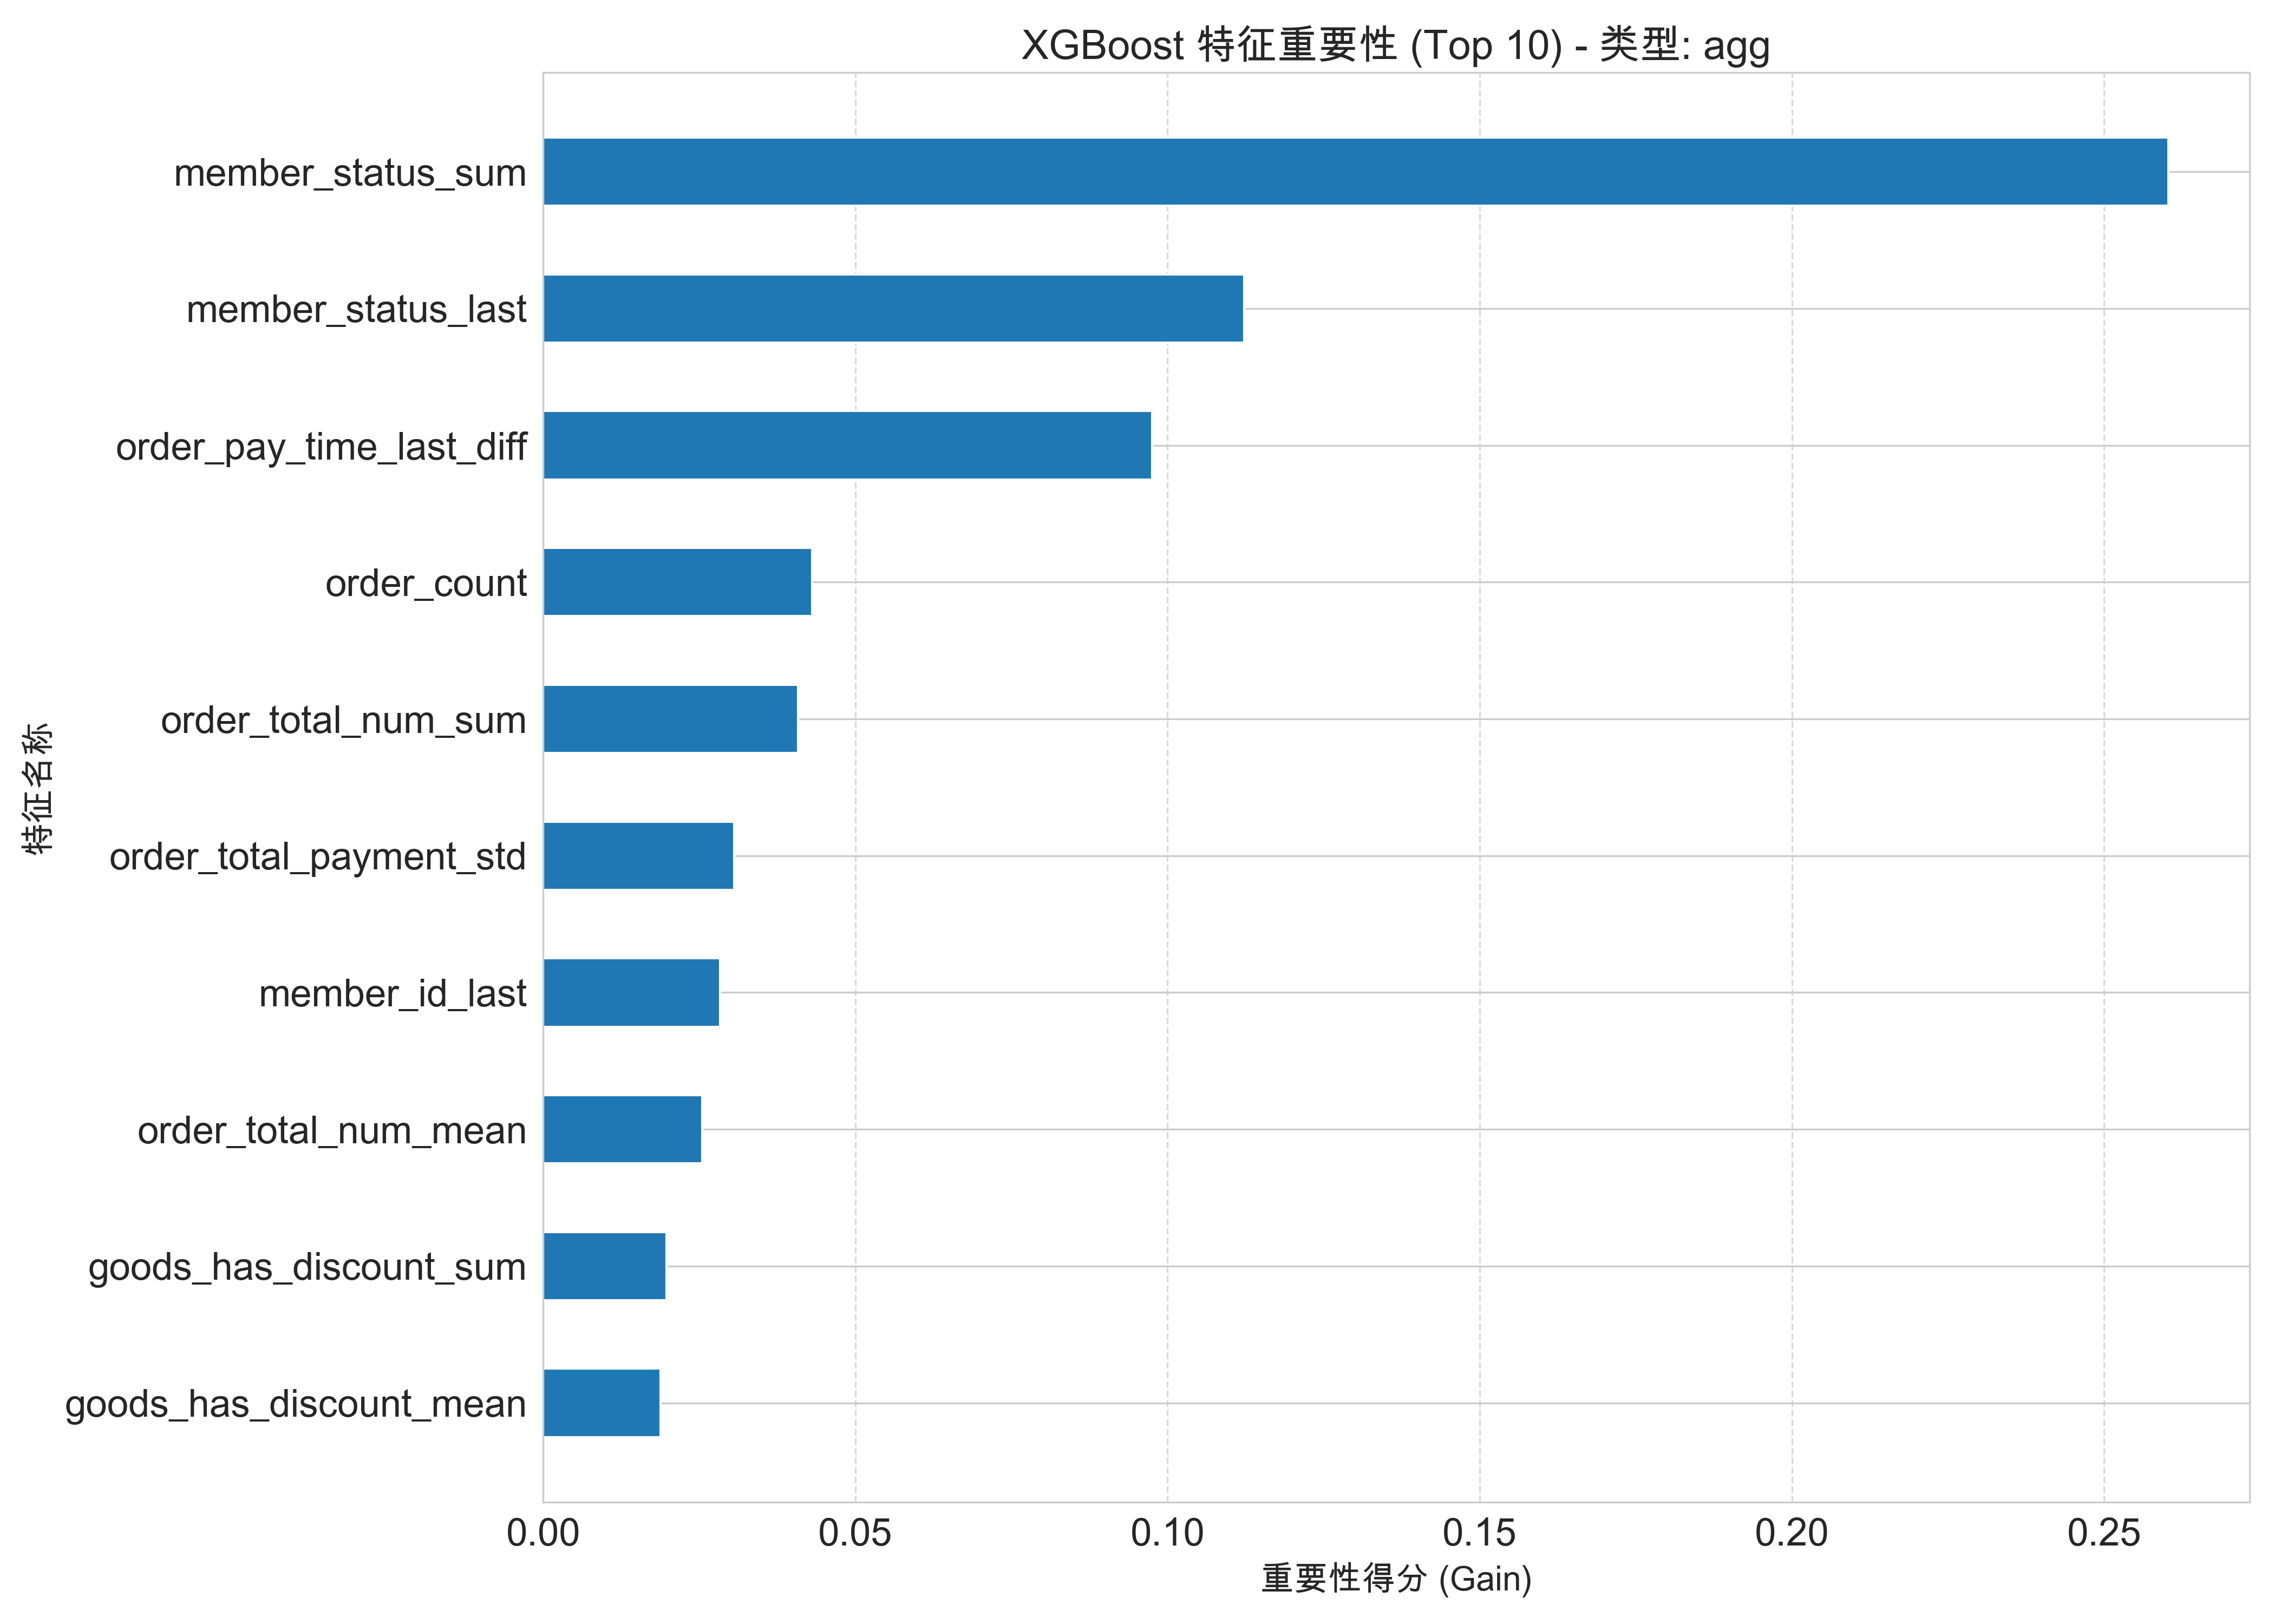
\includegraphics[width=\textwidth]{../analysis/xgb_agg_feature_importance.png}
    \caption{XGBoost模型在\texttt{agg}特征集上的特征重要性}
    \label{fig:xgb_agg}
\end{figure}

\begin{figure}[H]
    \centering
    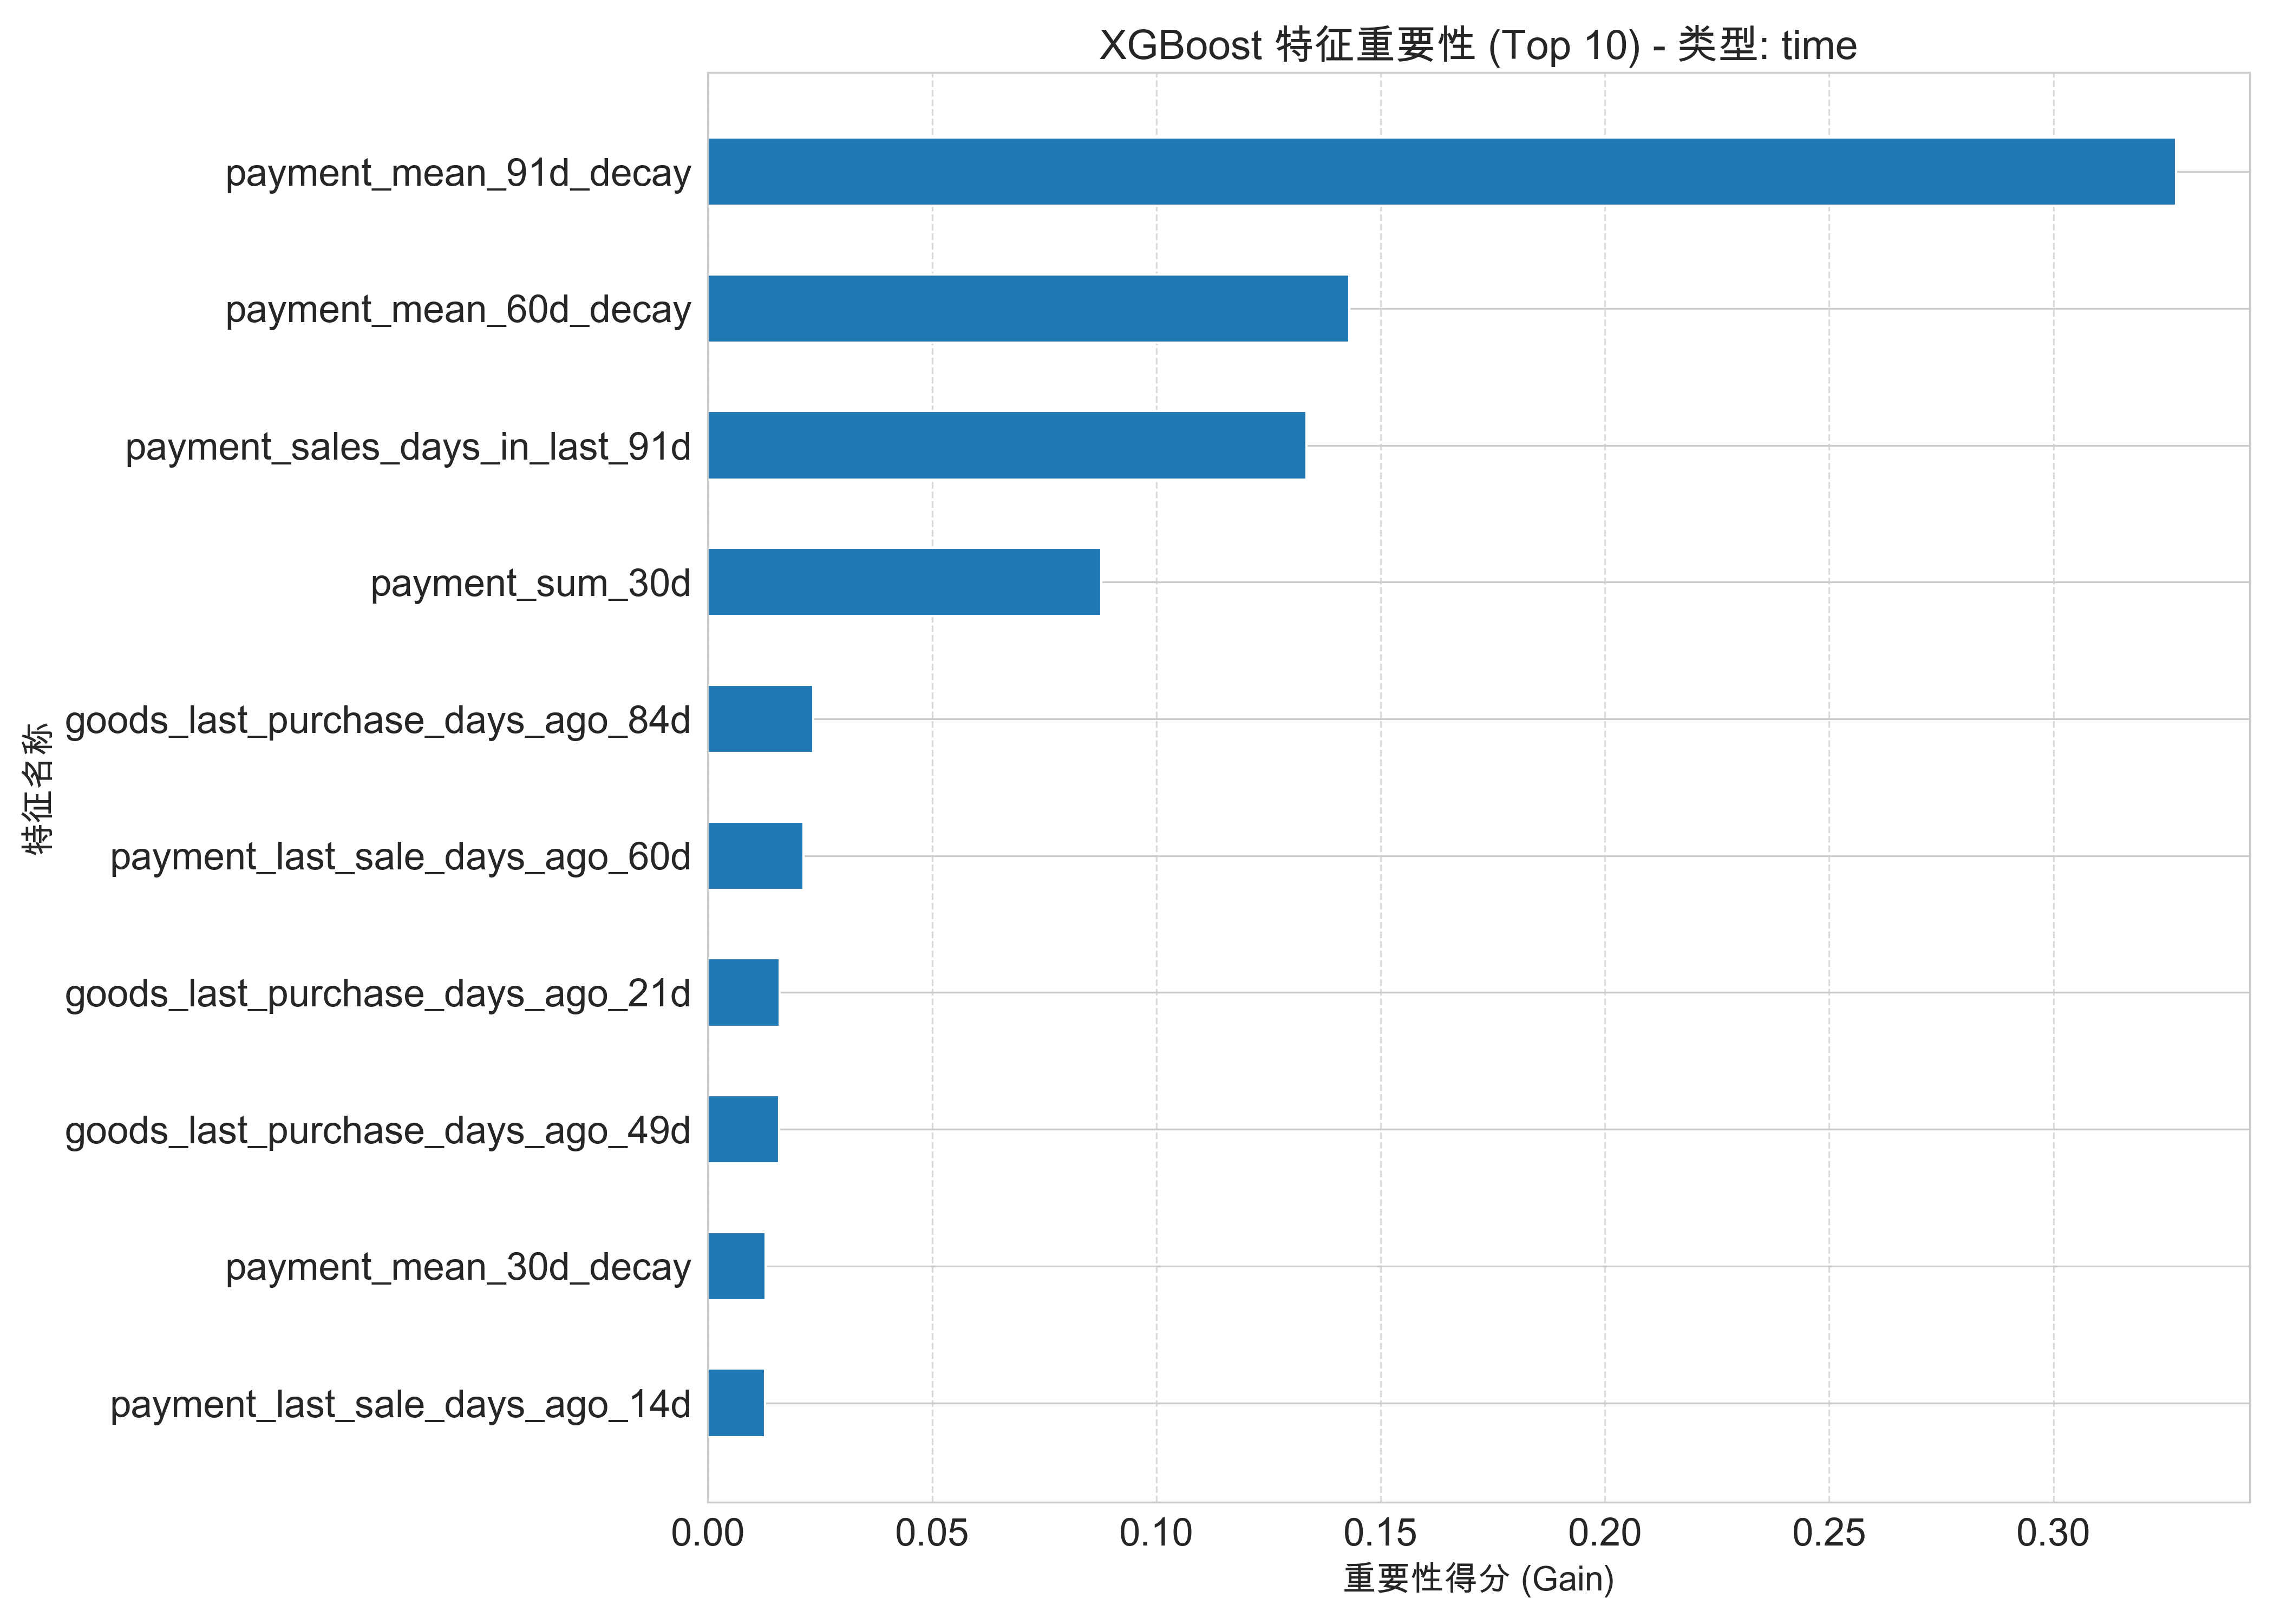
\includegraphics[width=\textwidth]{../analysis/xgb_time_feature_importance.png}
    \caption{XGBoost模型在\texttt{time}特征集上的特征重要性}
    \label{fig:xgb_time}
\end{figure}


\subsection{结论}
\begin{enumerate}
    \item \textbf{特征工程层面}: \textbf{静态聚合 + 动态时序} 的特征工程策略是预测用户购买行为的最优解. 静态画像是基础, 动态时序是精修.
    \item \textbf{算法层面}: \textbf{GBDT(XGBoost/LightGBM)} 是处理此类表格数据预测任务的最佳选择, 其强大的非线性建模能力和鲁棒性使其显著优于线性和神经网络模型.
\end{enumerate}

\end{document}